\chapter{\ifproject%
      \ifenglish Experimentation and Results\else การทดลองและผลลัพธ์\fi
  \else%
      \ifenglish System Evaluation\else การประเมินระบบ\fi
  \fi}


\section{Classification model}
\par ผลลัพธ์ จากการ train \& validation ด้วย 3546 sample เป็นจำนวน 200 Epoch

ตัวอย่าง ผลการทดลองของการ validation ด้วย 3546 sample
\begin{figure}[h]
    \begin{center}

        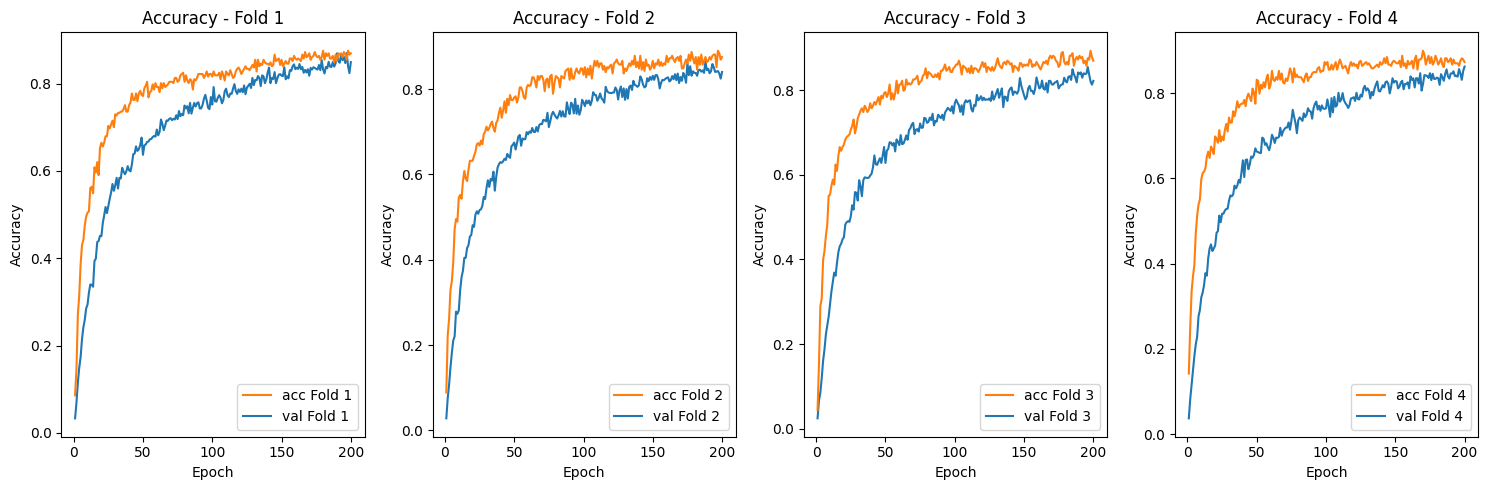
\includegraphics[scale=0.4]{pic/model/train_fold.png}
    \end{center}

    \caption[Train fold]{Train fold}
    \label{fig:Train fold}
\end{figure}

% โดยเมื่อนำ evaluate มาหา cross_entropy 0.23343226313591003, 0.944695234298706 accuracy

และทำการเลือก model ที่มีค่า Validation Score สูงสุดจากใน 4 model
เพื่อนำไปทำการ Blind Test
โดยได้นำ model ใน  Fold 4   มาทำการ
Evaluate (Blind Test)
\begin{align}
    \text{cross\_entropy} & = 1.175 \\
    \text{accuracy}       & = 0.72
\end{align}

Blind Test

\begin{figure}[h]
    \begin{center}

        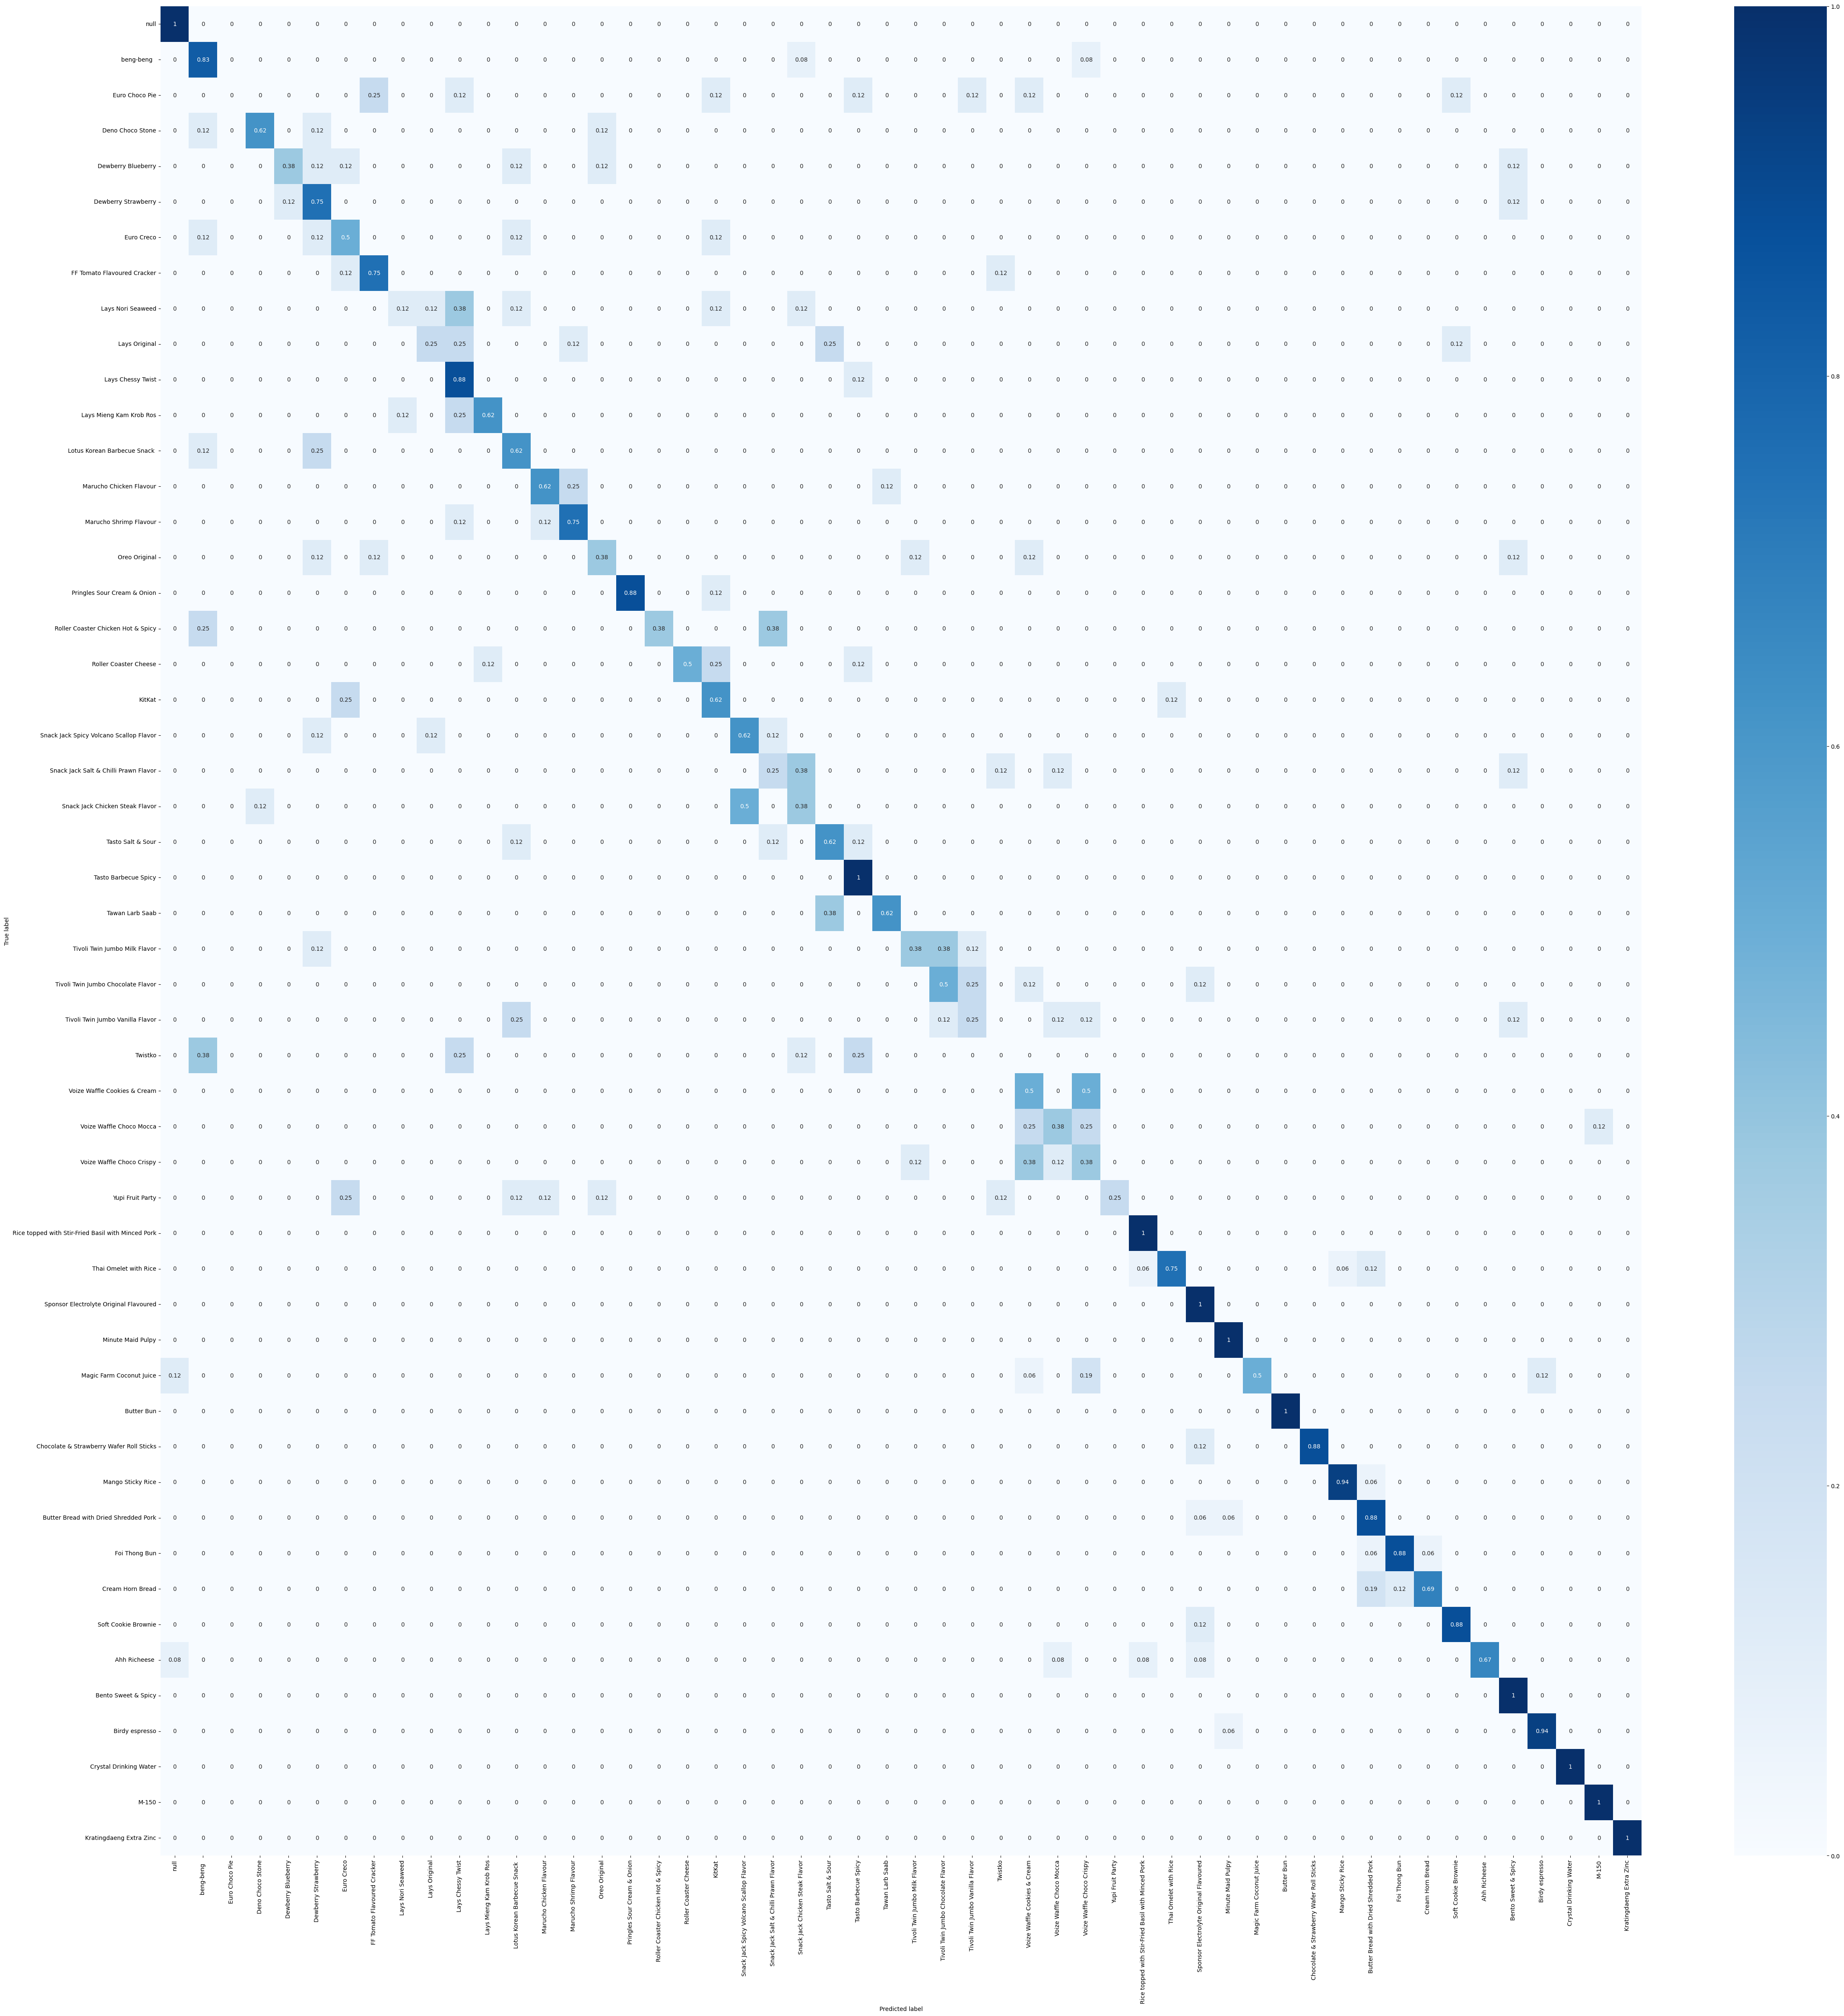
\includegraphics[scale=0.1]{pic/model/blind_pic_4_ccm.png}
    \end{center}

    \caption[Confusion matrix]{Confusion matrix}
    \label{fig:Confusion matrix}
\end{figure}




\newpage
\section{ผลการทำงานของระบบแอปพลิเคชันบนโทรศัพท์มือถือ}

% \begin{figure}[h]
%     \begin{center}

%     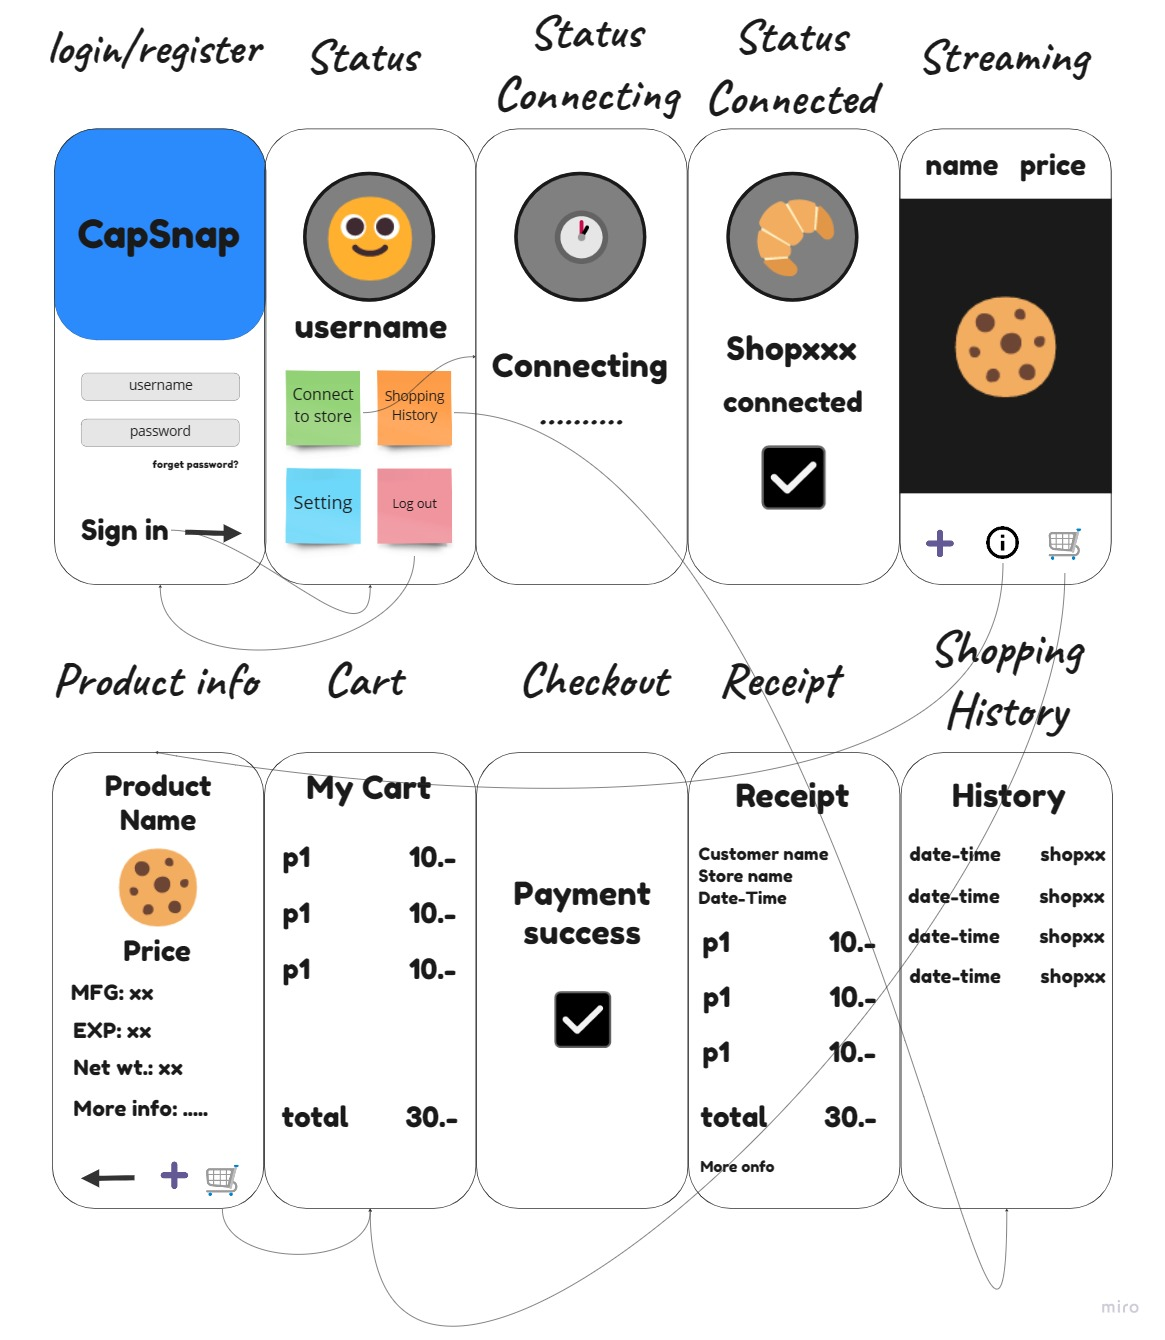
\includegraphics[scale=0.25]{pic/ui/mobileui.jpg}
%     \end{center}

%     \caption[Application wire frame]{Application wire frame}
%     \label{fig:Application wire frame}
%     \end{figure} 

ในส่วนของการออกแบบส่วนสื่อประสานกับผู้ใช้ (GUI) ของแอพลิเคชันมือถือนั้น ได้กำหนดให้มีหน้าการใช้งานหลักทั้งหมด 7 หน้า ได้แก่

\begin{enumerate}
    \item Login page: หน้าการเข้าสู่ระบบ
    \item Register page: หน้าลงทะเบียนเข้าใช้งาน
    \item Home page: หน้าแสดงชื่อผู้ใช้ และเมนูของฟังก์ชันต่าง ๆ
    \item Streaming page: หน้าฟังก์ชันการสตรีมมิ่งรูปภาพสินค้าผ่านกล้องมือถือแบบเรียลไทม์ ซึ่งจะแสดงชื่อ และราคาของสินค้า ซึ่งมีปุ่มการทำงานดังนี้ ปุ่มกดดูรายละเอียดสินค้า ,  ปุ่มเพิ่มสินค้าลงตะกร้า , ปุ่มกดดูสินค้าในตะกร้า
    \item Product Stock page: หน้าแสดงรายละเอียดของสินค้า
    \item My cart page: หน้าแสดง และจัดการเพิ่ม-ลบสินค้าในตะกร้า
    \item History page: หน้าแสดงประวัติการซื้อสินค้า
\end{enumerate}

\begin{figure}
    \begin{center}
        \begin{tabular}{c@{\hspace{3cm}}c}

            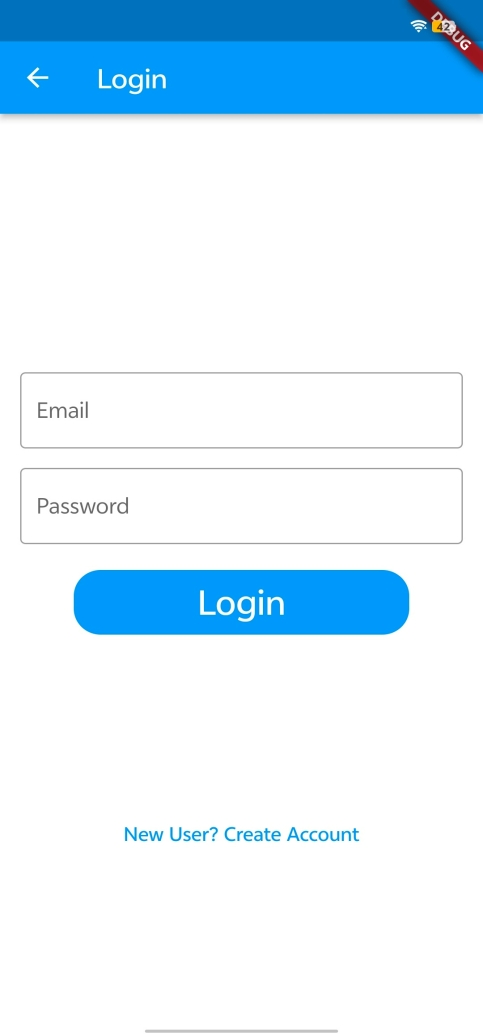
\includegraphics[scale=0.4]{pic/moblie/login.jpg}   & 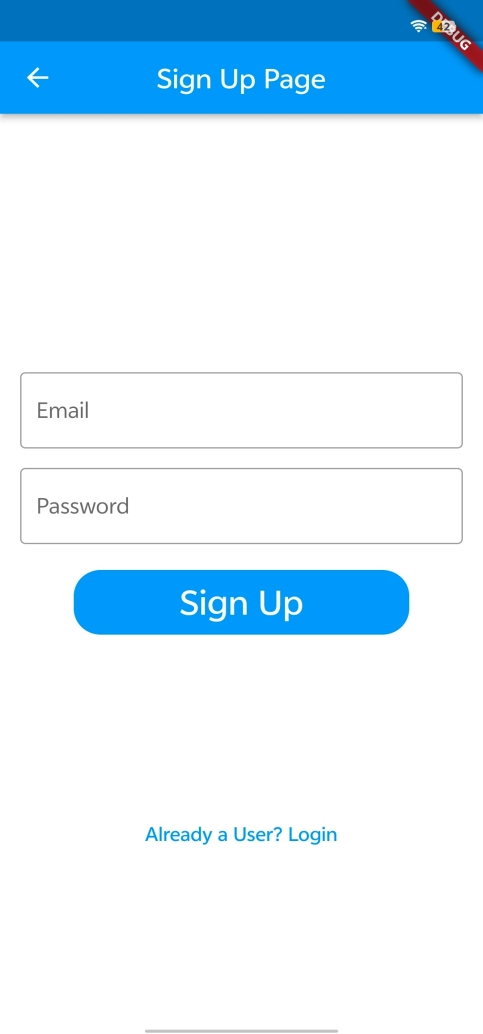
\includegraphics[scale=0.4]{pic/moblie/signup.jpg} \\
            Login                                               & Signup                                             \\[6pt]

            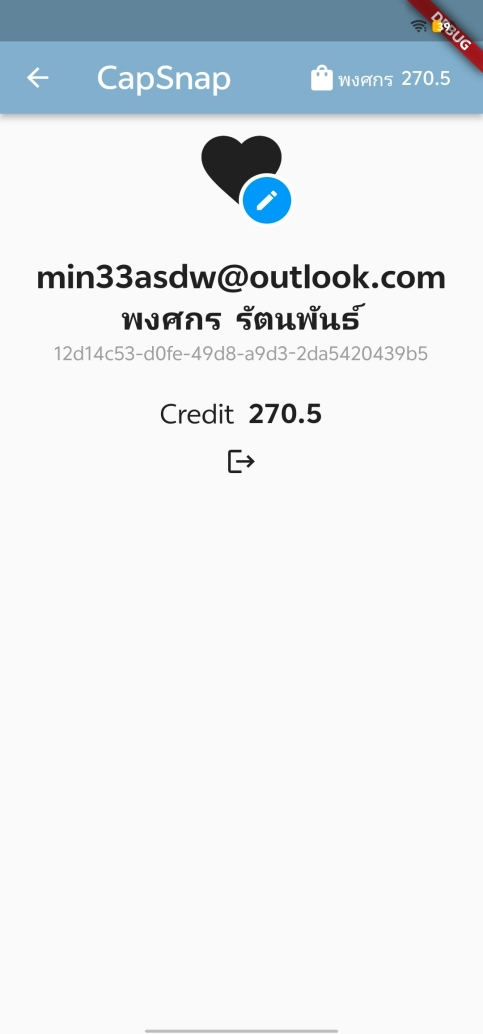
\includegraphics[scale=0.4]{pic/moblie/profile.jpg} & 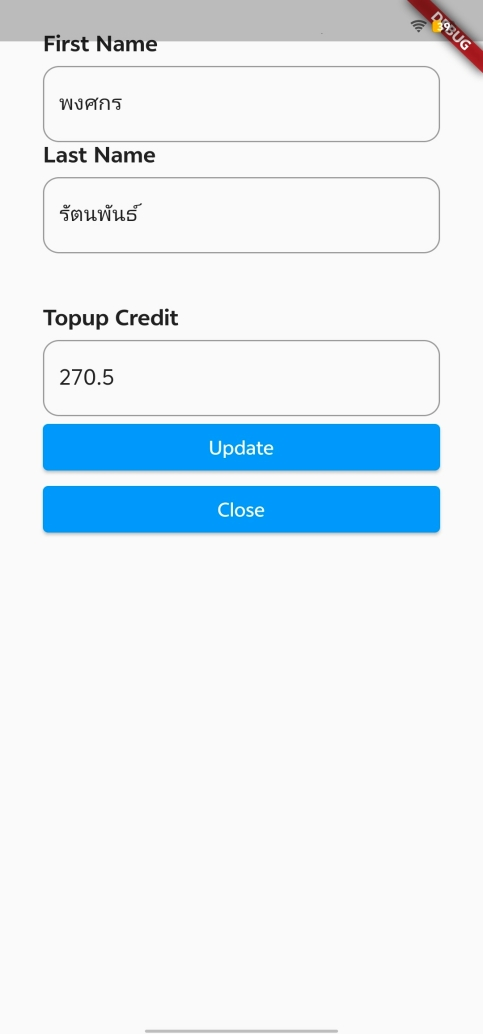
\includegraphics[scale=0.4]{pic/moblie/edit.jpg}   \\
            Profile                                             & Edit profile                                       \\[6pt]
        \end{tabular}
    \end{center}
\end{figure}

\begin{figure}
    \begin{center}
        \begin{tabular}{c@{\hspace{3cm}}c}

            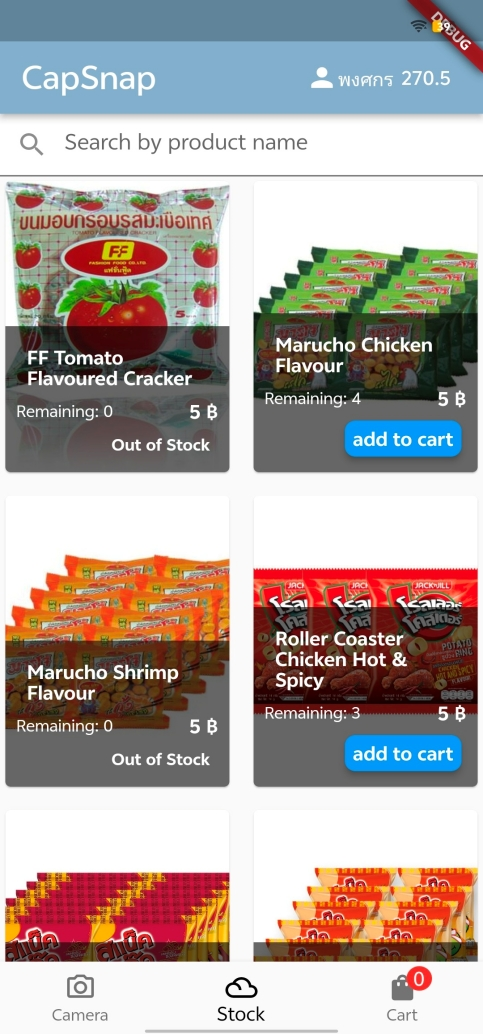
\includegraphics[scale=0.4]{pic/moblie/stock.jpg}        & 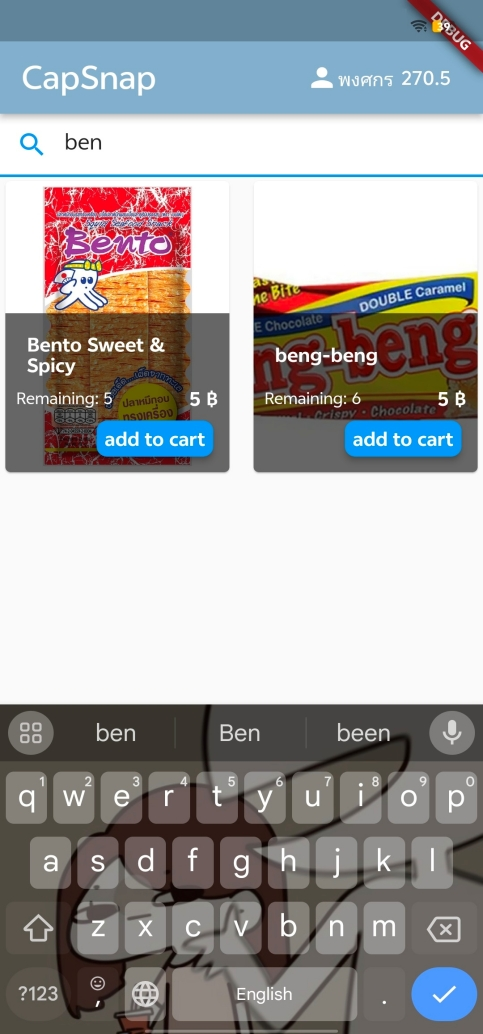
\includegraphics[scale=0.4]{pic/moblie/search_products.jpg} \\
            Stock                                                    & Search products                                             \\[6pt]

            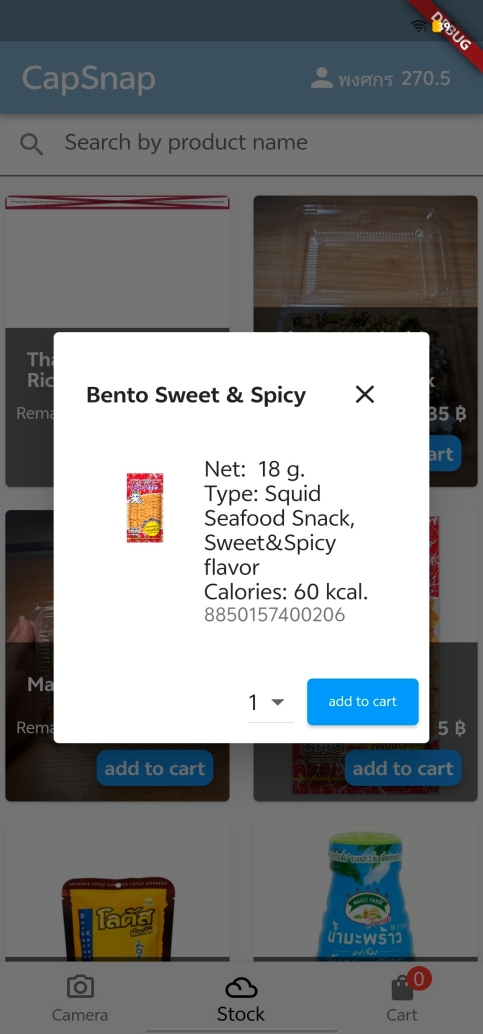
\includegraphics[scale=0.4]{pic/moblie/stock_detail.jpg} & 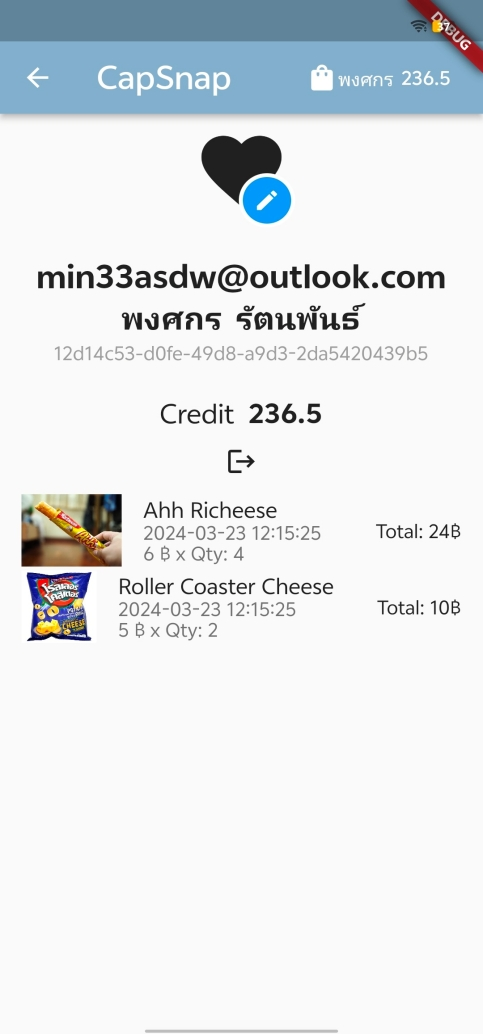
\includegraphics[scale=0.4]{pic/moblie/history.jpg}         \\
            Product detail                                           & Purchase history                                            \\[6pt]
        \end{tabular}
    \end{center}
\end{figure}

\begin{figure}
    \begin{center}
        \begin{tabular}{c@{\hspace{3cm}}c}

            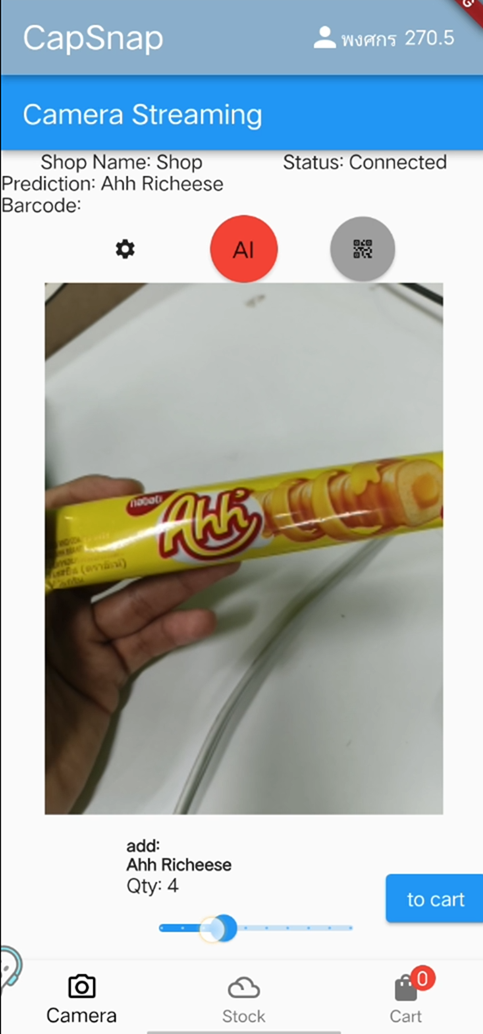
\includegraphics[scale=0.4]{pic/moblie/camera_ai.png} & 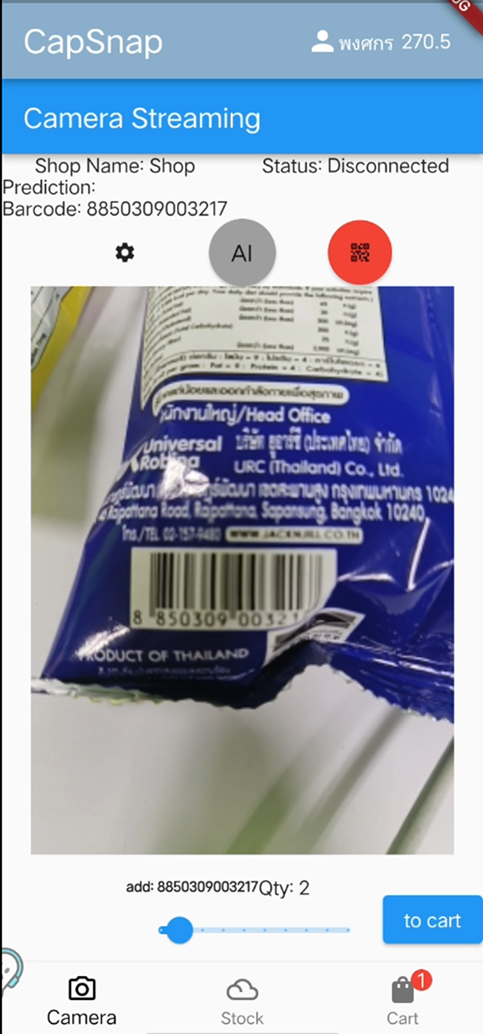
\includegraphics[scale=0.4]{pic/moblie/camera_barcode.png} \\
            Camera streaming                                      & Camera barcode                                             \\[6pt]

            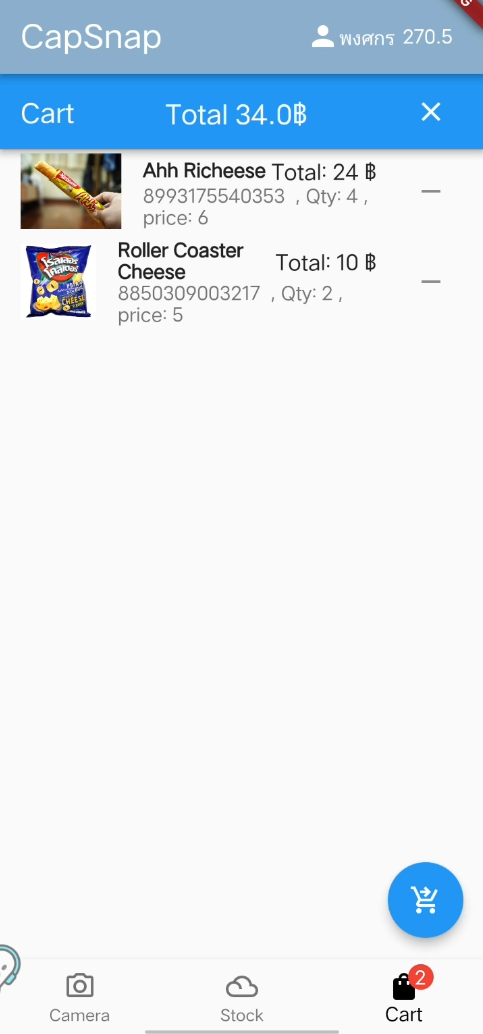
\includegraphics[scale=0.4]{pic/moblie/cart.png}      & 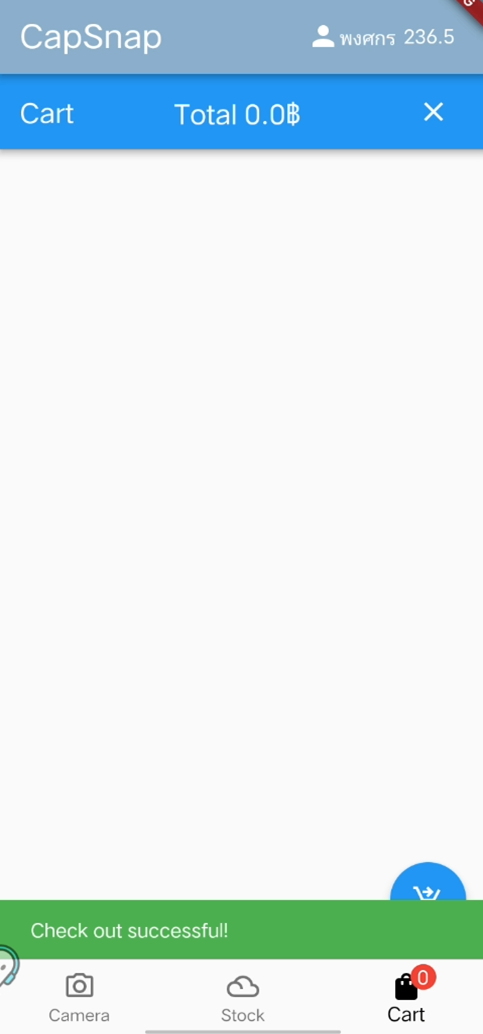
\includegraphics[scale=0.4]{pic/moblie/checkout.png}       \\
            Cart                                                  & Checkout                                                   \\[6pt]
        \end{tabular}
    \end{center}
\end{figure}
% \begin{figure}[h]
%     \begin{center}

%         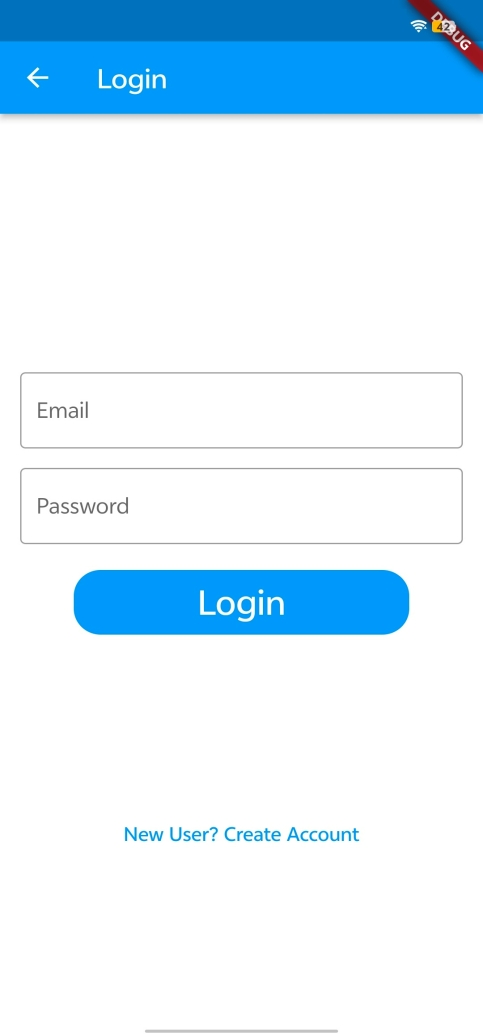
\includegraphics[scale=0.1]{pic/moblie/login.jpg}
%     \end{center}

%     \caption[App Login]{App Login}
% \label{fig:App Login}
% \end{figure} 

% \begin{figure}[h]
%     \begin{center}

%         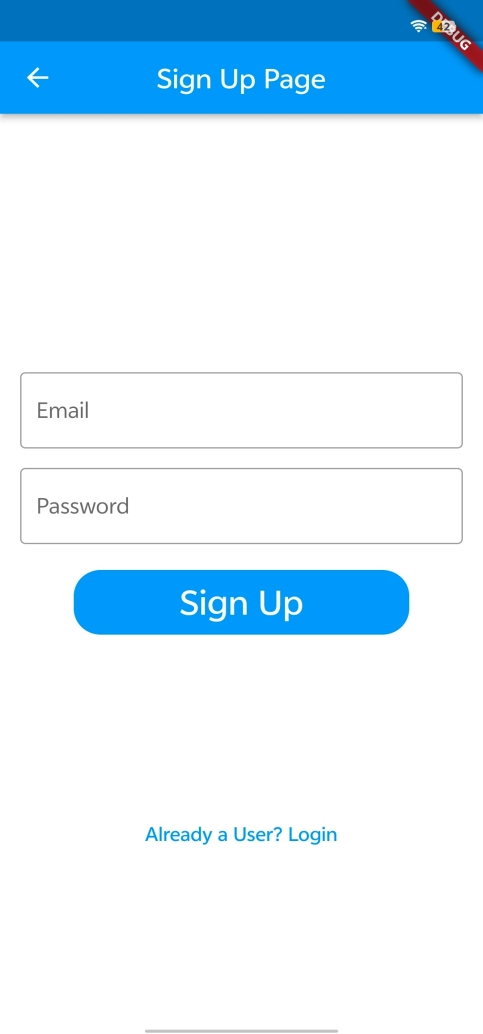
\includegraphics[scale=0.1]{pic/moblie/signup.jpg}
%     \end{center}

%     \caption[App signup]{App signup}
% \label{fig:App signup}
% \end{figure} 

% \begin{figure}[h]
%     \begin{center}

%         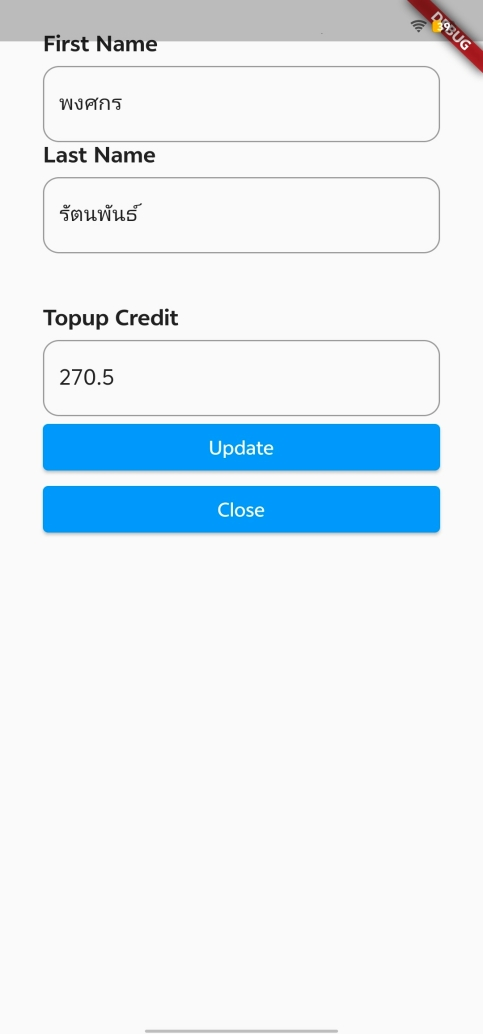
\includegraphics[scale=0.1]{pic/moblie/edit.jpg}
%     \end{center}

%     \caption[App edit]{App edit}
% \label{fig:App edit}
% \end{figure} 
\newpage
\section{ผลการ checkout}
จากการทดลองและบันทึกผลของเรา ทำการบันทึกข้อมูลและค่าเฉลี่่ยได้ดังนี้
(ขึ้นอยู่กับผู้ใช้งานแต่ละคน)
\begin{table}[]
    \centering
    \caption{Camera classification process}
    \begin{tabular}{|p{5cm}|p{4cm}|p{4cm}|}
        \hline
        \textbf{Camera Classification} & \textbf{ซื้อของ 1 ชิ้น (วินาที)} & \textbf{ซื้อของ 5 ชิ้น (วินาที)} \\
        \hline
        Camera streaming               & 2-5 s                         & 10-25 s                       \\
        Image processing               & 1-2 s                         & 5-10 s                        \\
        Payment transaction            & 2 s                           & 2 s                           \\
        \hline
        Total Time Usage               & 5-9 s                         & 17-37 s                       \\
        \hline
    \end{tabular}
\end{table}


\begin{table}[]
    \centering
    \caption{Camera barcode process}
    \begin{tabular}{|p{5cm}|p{4cm}|p{4cm}|}
        \hline
        \textbf{Barcode payment} & \textbf{ซื้อของ 1 ชิ้น (วินาที)} & \textbf{ซื้อของ 5 ชิ้น (วินาที)} \\
        \hline
        Camera capture           & 2-5 s                         & 10-25 s                       \\
        Barcode processing       & 0.5 s                         & 2.5 s                         \\
        Payment transaction      & 2 s                           & 2 s                           \\
        \hline
        Total Time Usage         & 2.5-7 s                       & 14.5-29.5 s                   \\
        \hline
    \end{tabular}
\end{table}


\begin{table}[]
    \centering
    \caption{Line Checkout process}
    \begin{tabular}{|p{5cm}|p{4cm}|p{4cm}|}
        \hline
        \textbf{Line Checkout Cashier} & \textbf{ซื้อของ 1 ชิ้น(seconds)} & \textbf{ซื้อของ 5 ชิ้น (seconds)} \\
        \hline
        Waiting in line                & 30-120 s                     & 30-120 s                      \\
        Cashier processing             & 10-20 s                      & 20-40 s                       \\
        Payment transaction            & 5-10 s                       & 5-10 s                        \\
        \hline
        Total Time Usage               & 45-150 s                     & 55-170 s                      \\
        \hline
    \end{tabular}
\end{table}

\newpage
\section{ผลการทำงานของระบบเว็บไซต์สำหรับร้านค้า}
จากการปฏิบัติงาน สามารถพัฒนาระบบระบบเว็บไซต์สำหรับร้านค้าได้เสร็จสมบูรณ์ โดยสามารถแสดงผลการทำงานของหน้าเว็บไซต์แบ่งตามแต่ละหน้าของเว็บไซต์ได้ดังนี้
\begin{enumerate}
    \item หน้าลงชื่อเข้าใช้งาน (Login)
    \item หน้าการตั้งค่าร้านค้า และผู้ดูแลร้านค้า (Store Settings)
    \item หน้าการจัดการสินค้า (Stock Manager)
    \item หน้าแสดงรายงานยอดขายสินค้า (Selling Report)
    \item หน้าแสดงข้อมูลลูกค้า (Customers)
    \item หน้าแสดงประวัติการซื้อสินค้าของลูกค้า (Purchase History)
\end{enumerate}

\subsection{หน้าลงชื่อเข้าใช้งาน (Login)}
สำหรับหน้านี้ จะเป็นหน้าแรกของการเข้าใช้งานระบบ โดยสามารถลงชื่อเข้าใช้งานได้เท่านั้น แต่จะไม่สามารถลงทะเบียนได้ เนื่องจากผู้ใช้งานระบบ ต้องเป็นผู้ดูแลระบบร้านค้า หรือพนักงานของร้าน ซึ่งจะถูกเพิ่มโดย Super Administer ซึ่งอาจเป็นเจ้าของร้าน หรือผู้จัดการร้าน โดยผู้ใช้งานสามารถขอข้อมูลรหัสผ่านจาก Super Administer โดยตรงเพื่อนำมาใช้เข้าสู่ระบบ\\
{

\includegraphics[scale=0.35]{pic/ui/w26.png}
}\\
{
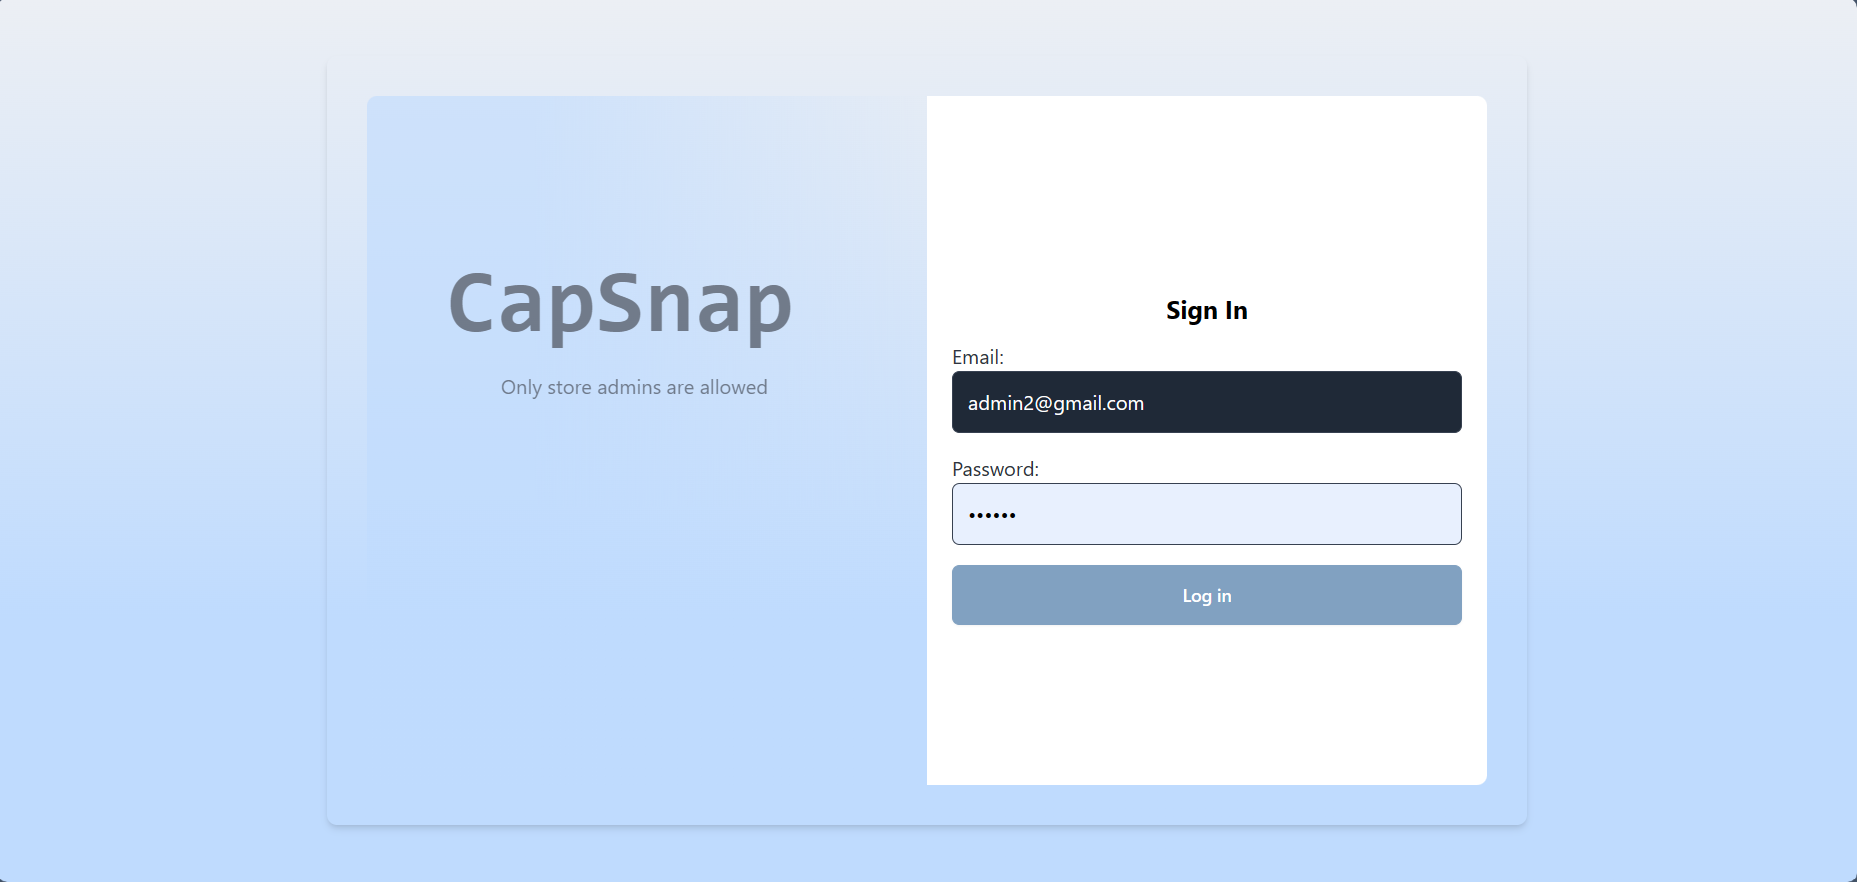
\includegraphics[scale=0.35]{pic/ui/w27.png}
}\\
{
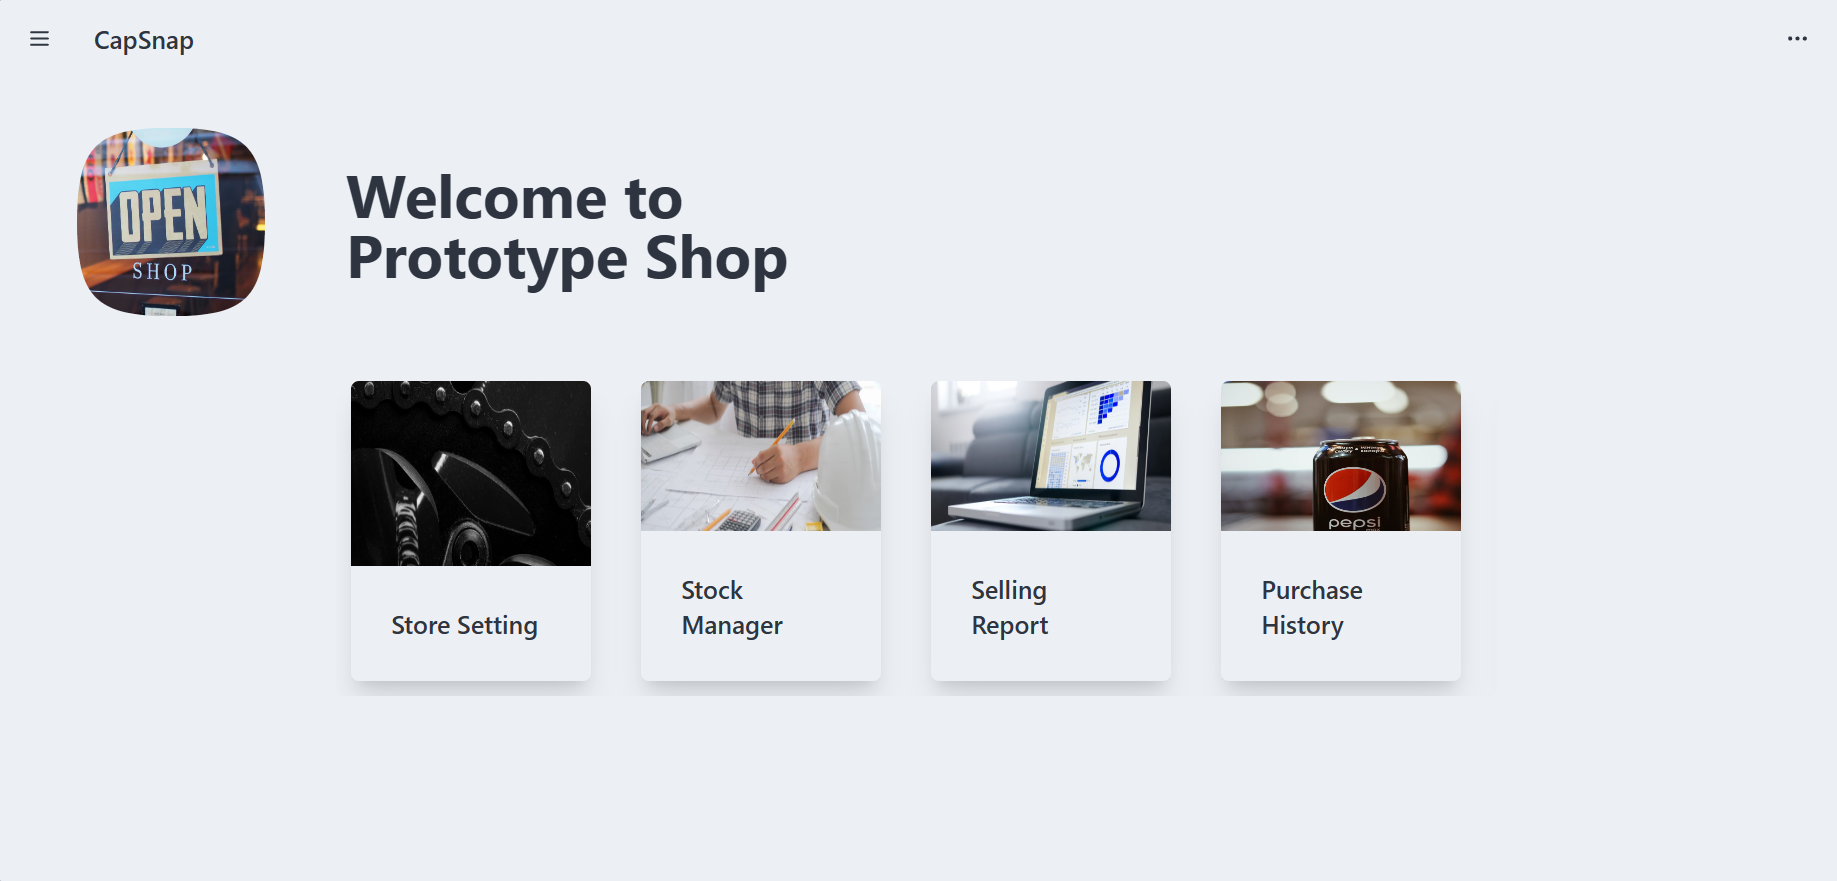
\includegraphics[scale=0.35]{pic/ui/w1.png}
}\\
{
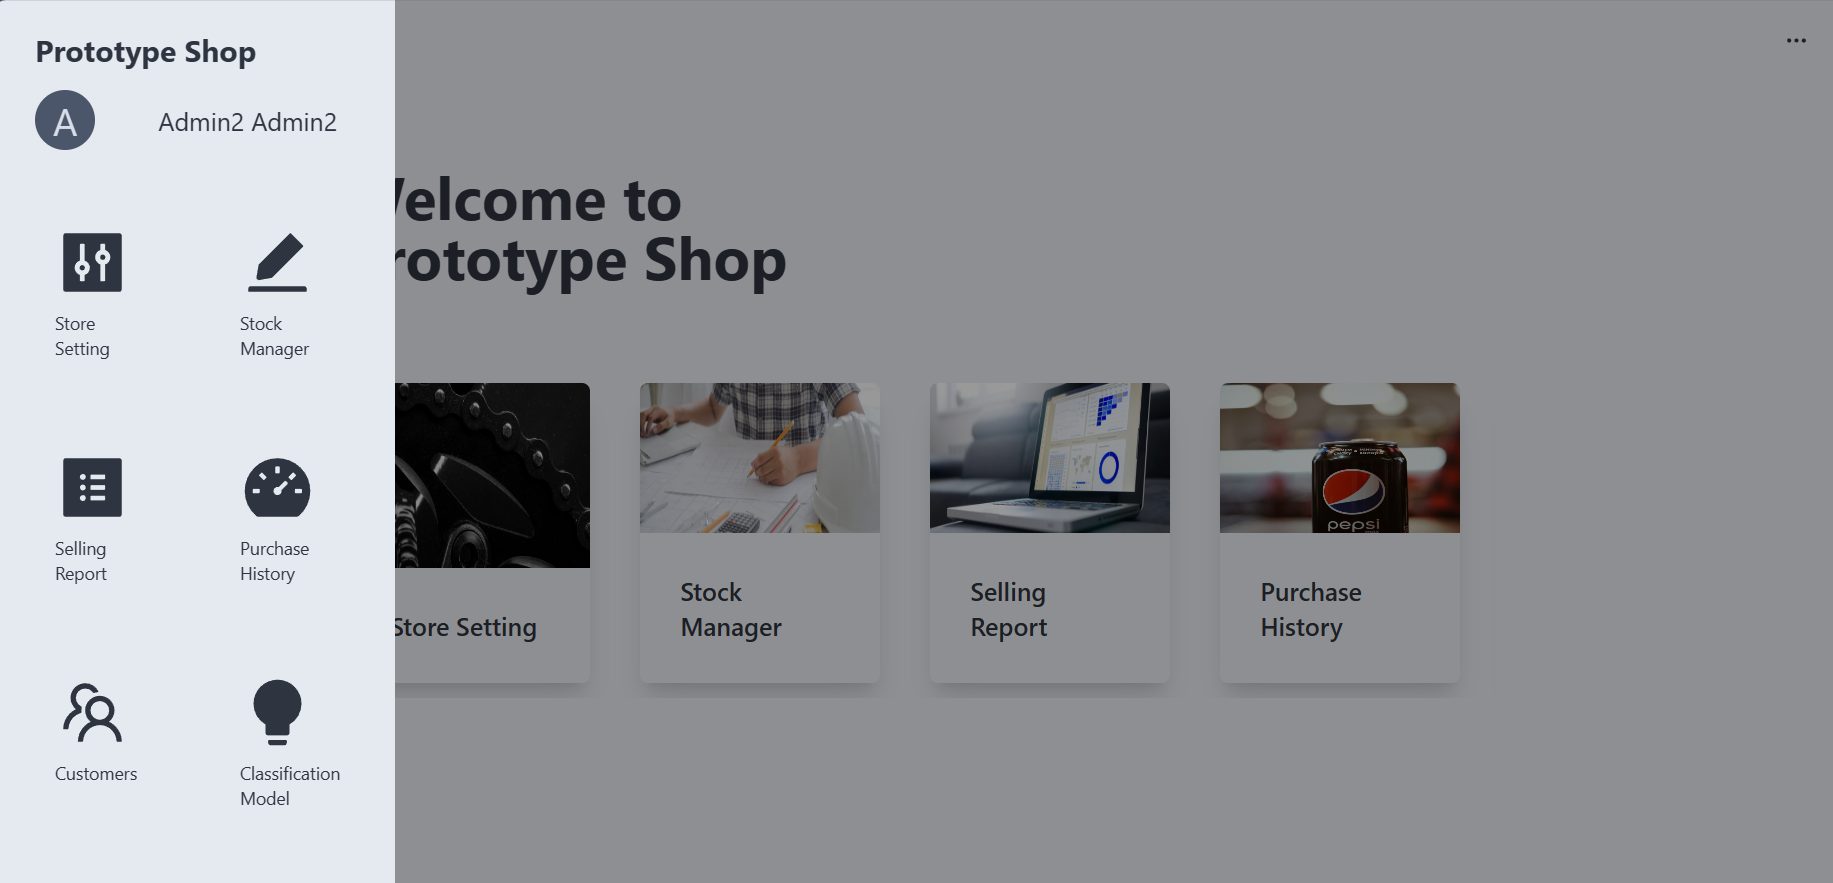
\includegraphics[scale=0.35]{pic/ui/w2.png}
}\\

\subsection{หน้าการตั้งค่าร้านค้า และผู้ดูแลร้านค้า (Store Settings)}
สำหรับหน้านี้ผู้ใช้งานสามารถตั้งค่าชื่อร้าน สถานที่ตั้ง และประเภทร้านค้าได้ รวมถึงเป็นหน้าการจัดการผู้ดูแลระบบ โดยการแสดงผลสามารถแบ่งได้เป็น 2 กรณีตามสถานะของผู้ใช้งาน ได้แก่
\begin{enumerate}
    \item Super Administer: สามารถดูรายชื่อ เพิ่ม หรือลบผู้ดูแลระบบร้านค้า (Administer) ได้ และสามารถแก้ไขมูลสถานะ และบทบาทของผู้ดูแลระบบร้านค้า และแก้ไขข้อมูลของตนเองได้
    \item Administer: สามารถดู และแก้ไขข้อมูลของตนเองได้เท่านั้น
\end{enumerate}
{
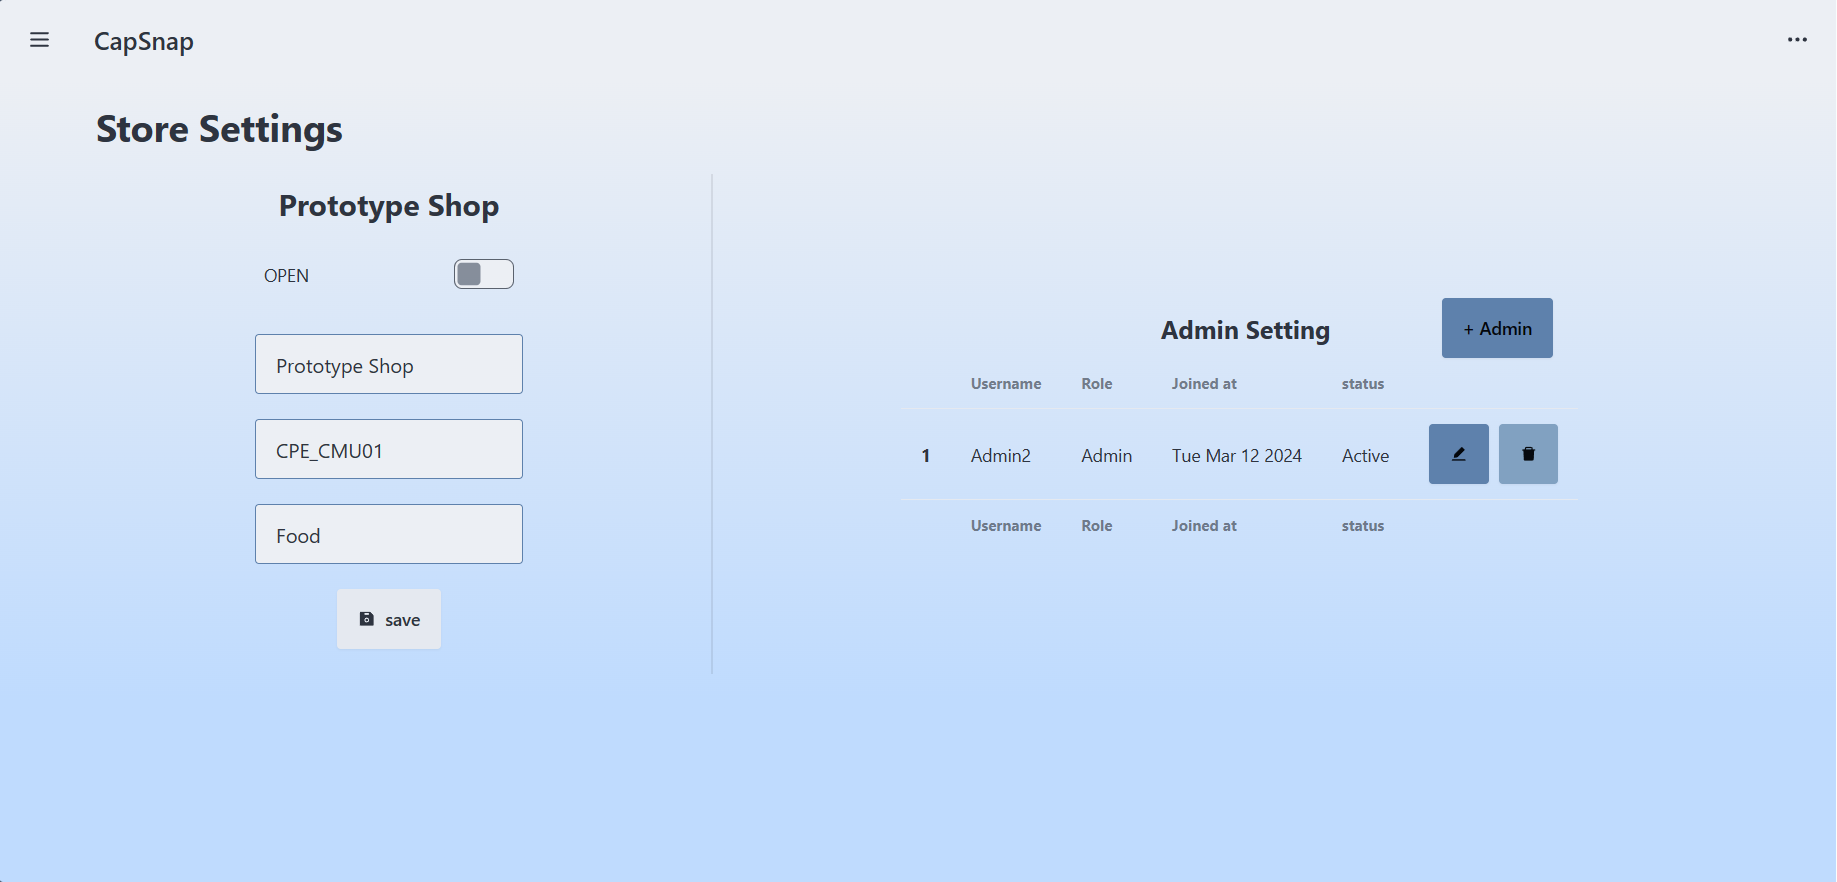
\includegraphics[scale=0.35]{pic/ui/w3.png}
}\\
\subsection{หน้าการจัดการสินค้า (Stock Manager)}
สำหรับหน้านี้จะแสดงรายการสินค้าทั้งหมดแยกตามหมวดหมู่ พร้อมข้อมูลทั้งหมด ได้แก่ ชื่อสินค้า รูปสินค้า ข้อมูลสินค้า ราคา จำนวนในคลัง และประวัติคลังสินค้า โดยสามารถทำการเพิ่ม ลบ และแก้ไขข้อมูลทั้งหมดได้ ดังนี้\\
{
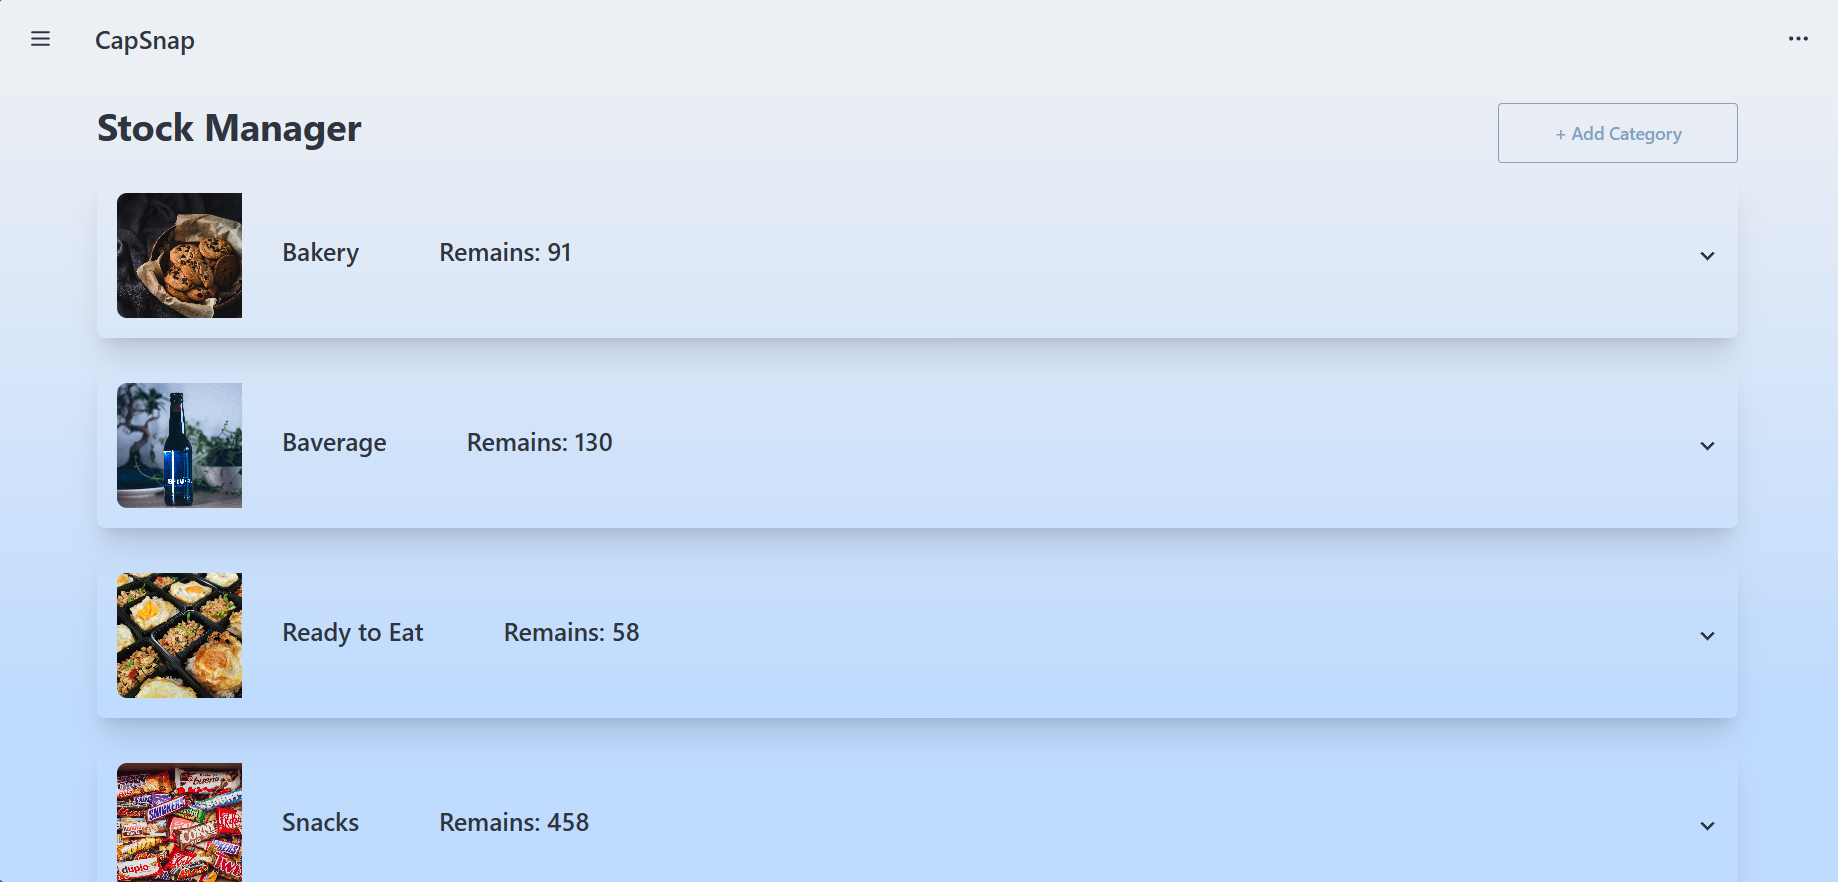
\includegraphics[scale=0.35]{pic/ui/w4.png}
}\\
{
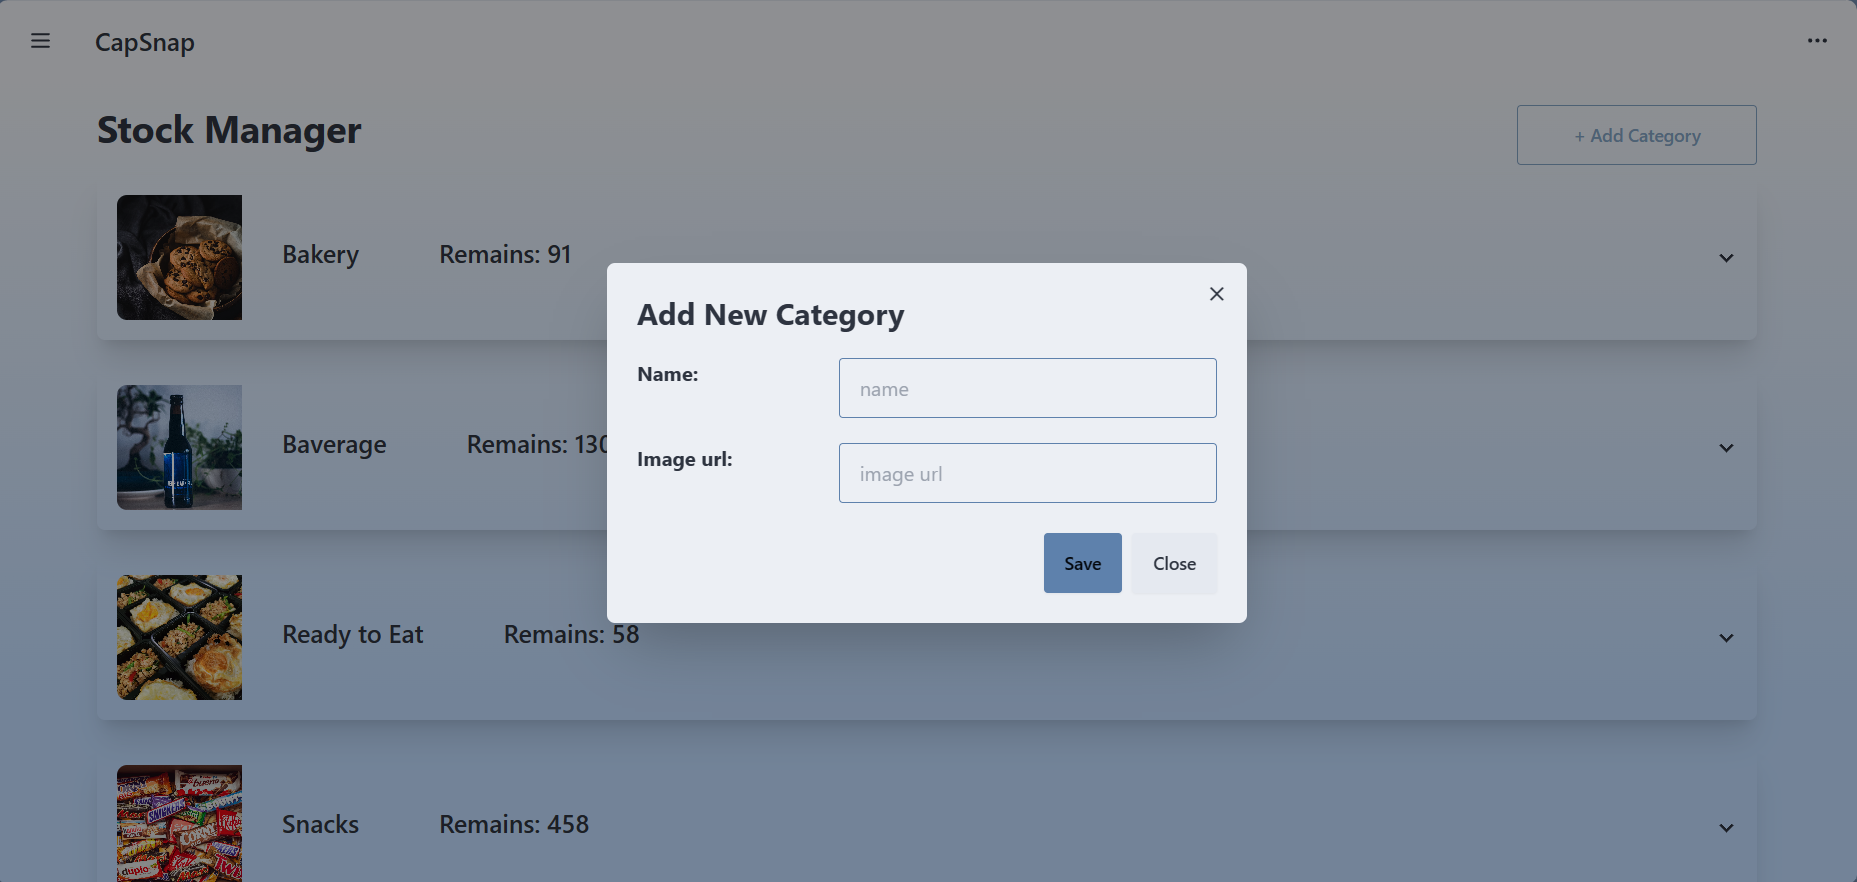
\includegraphics[scale=0.35]{pic/ui/w5.png}
% \includegraphics[scale=0.35]{pic/ui/w6.png}
}\\
{
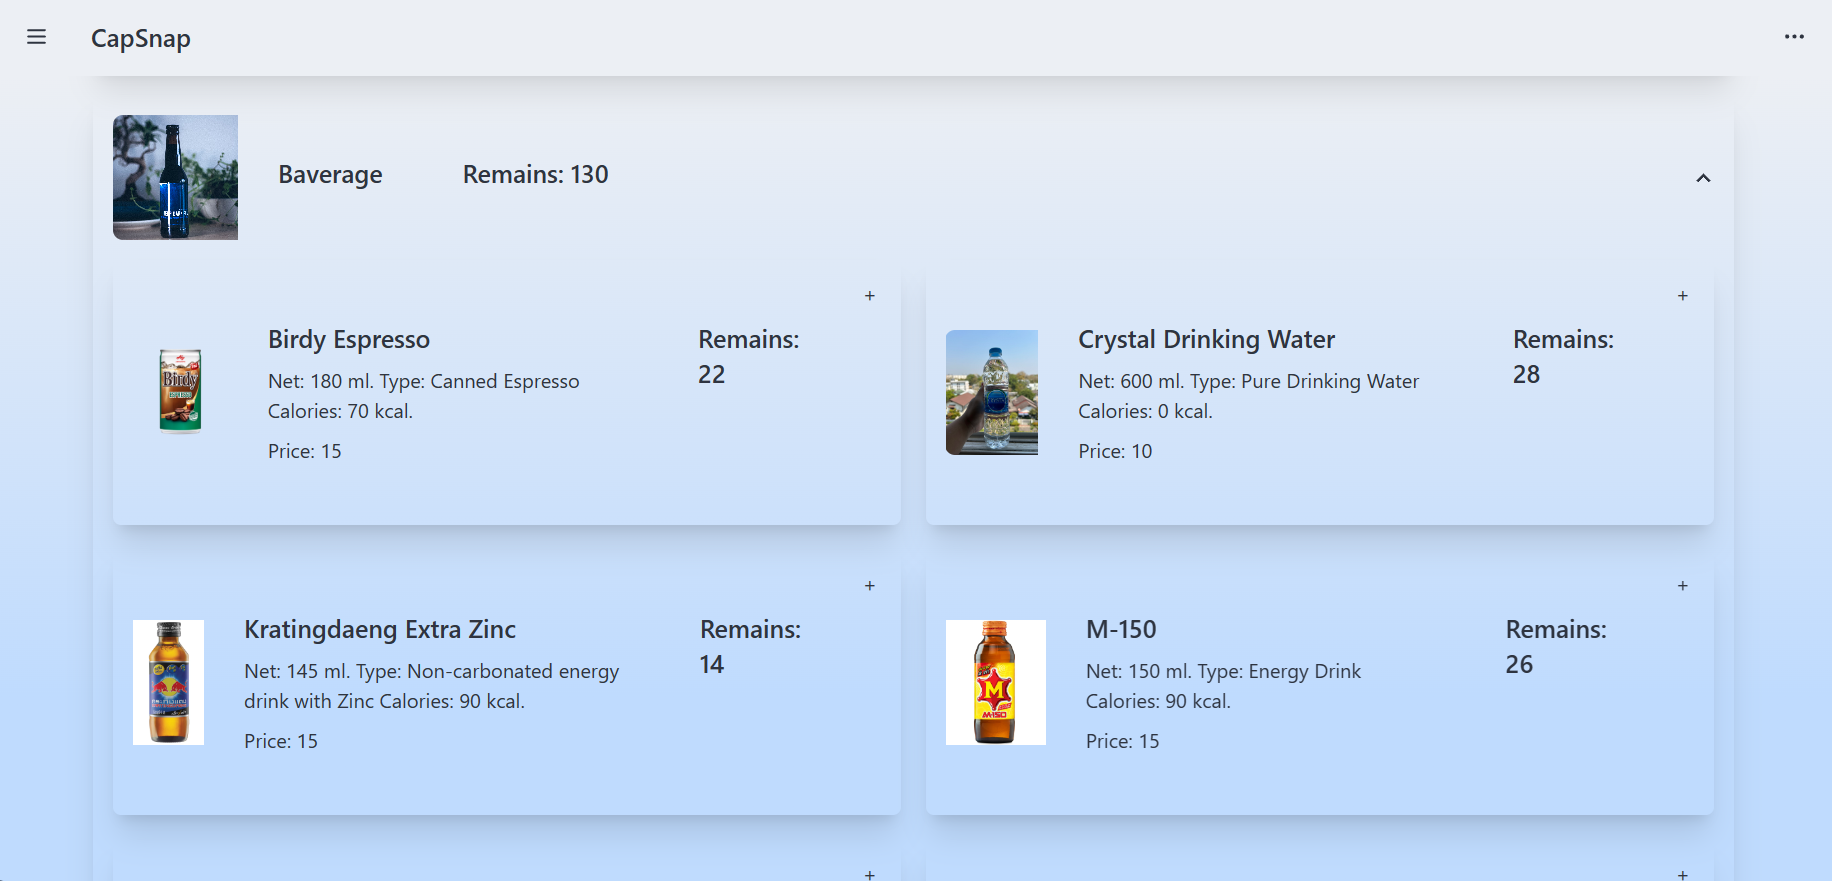
\includegraphics[scale=0.35]{pic/ui/w7.png}
}\\
{
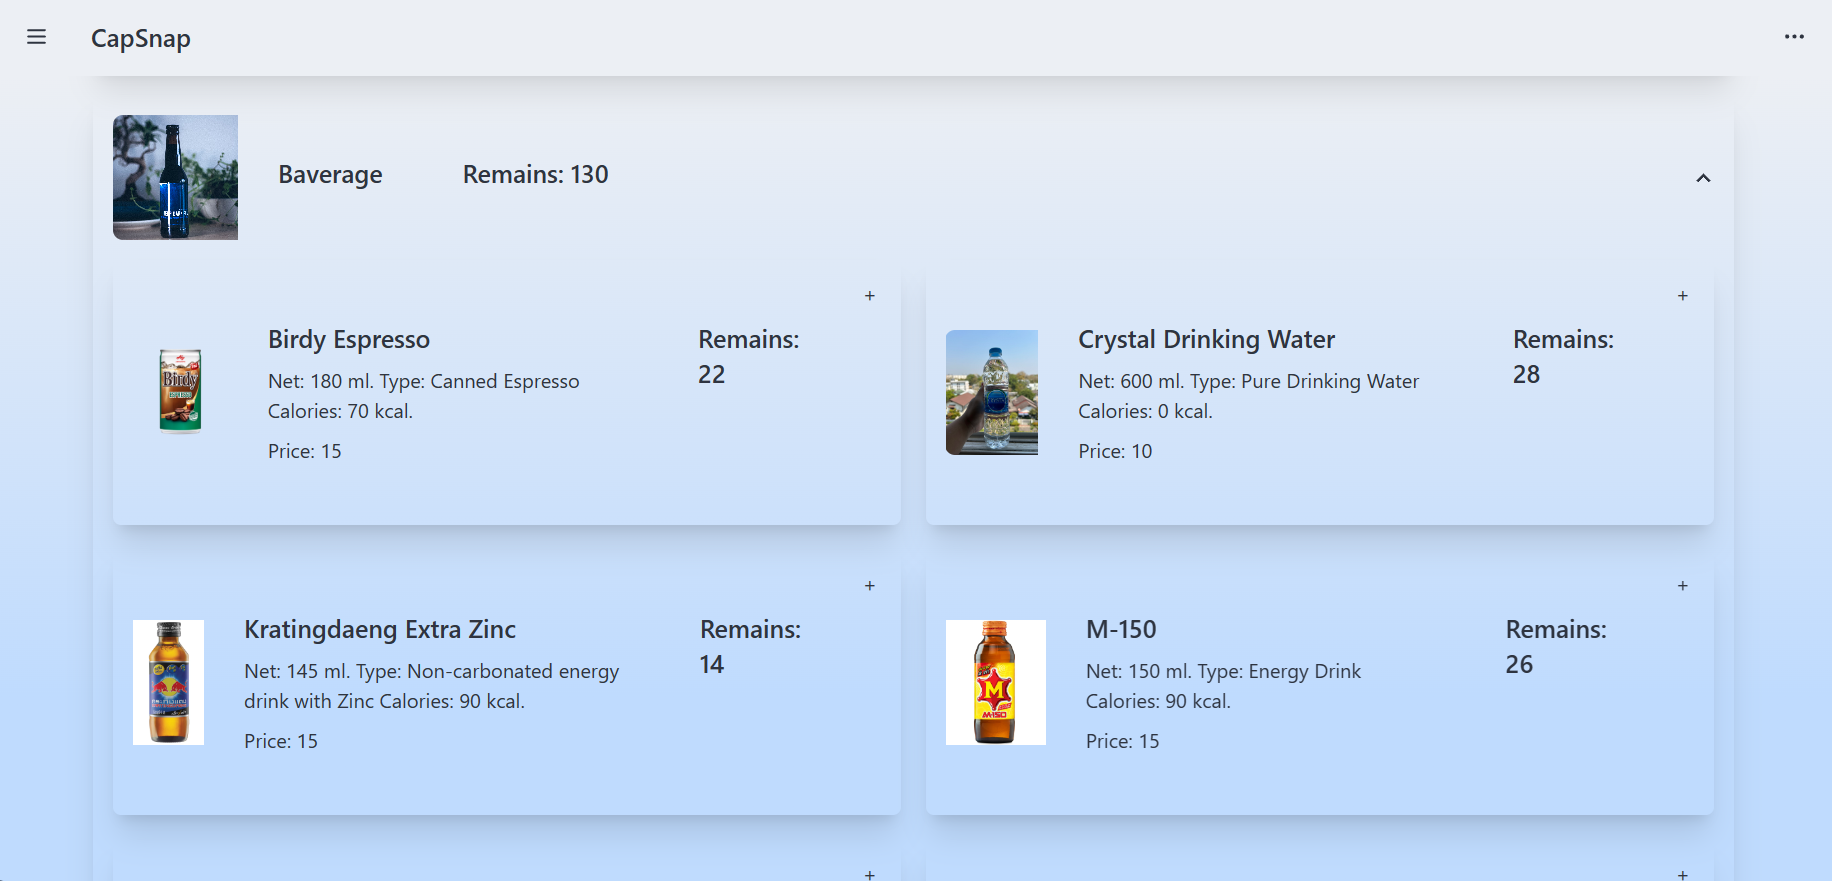
\includegraphics[scale=0.35]{pic/ui/w8.png}
}\\
{
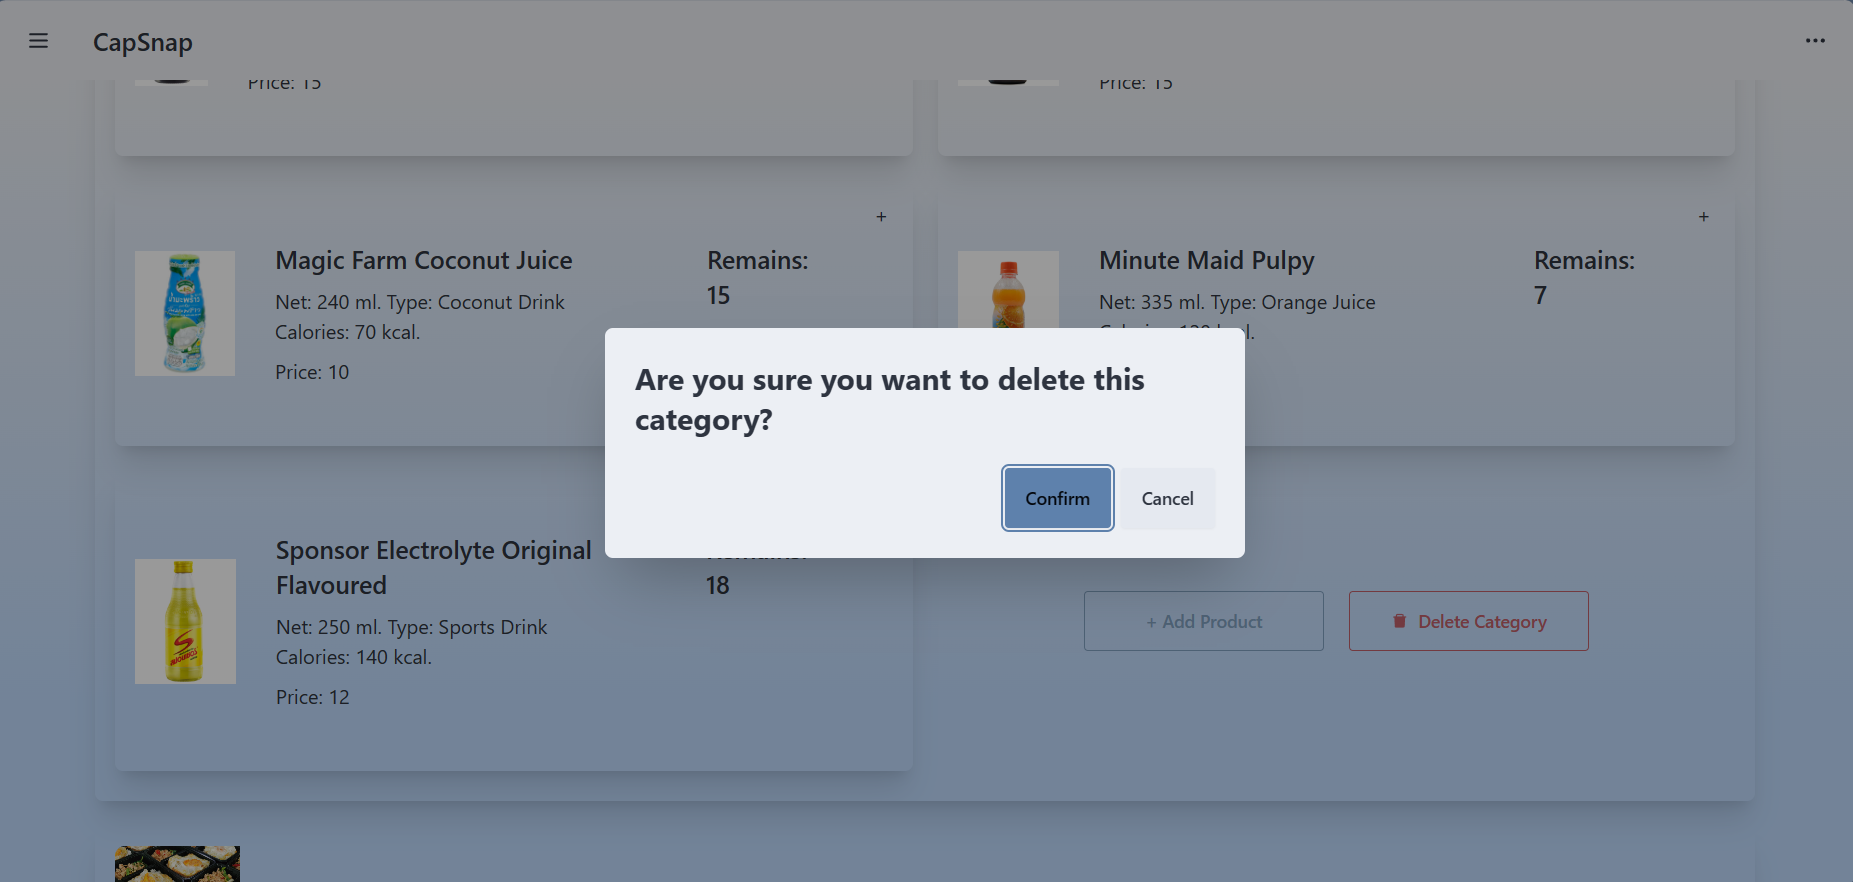
\includegraphics[scale=0.35]{pic/ui/w9.png}
}\\
{
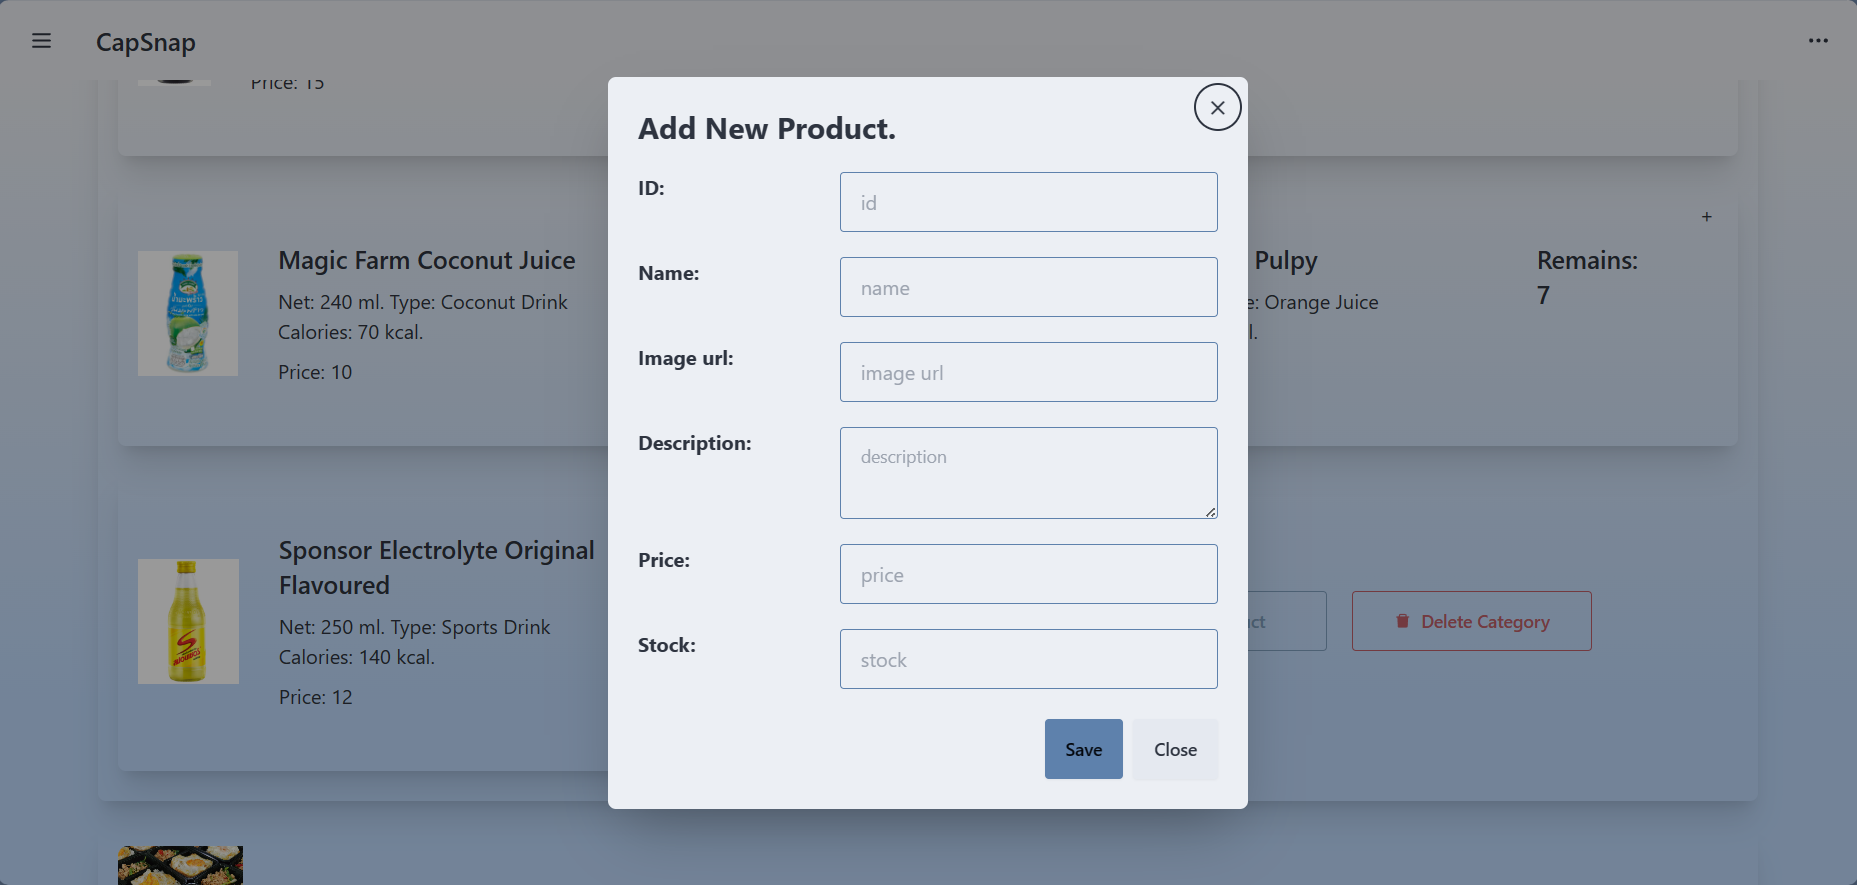
\includegraphics[scale=0.35]{pic/ui/w10.png}
}\\
{
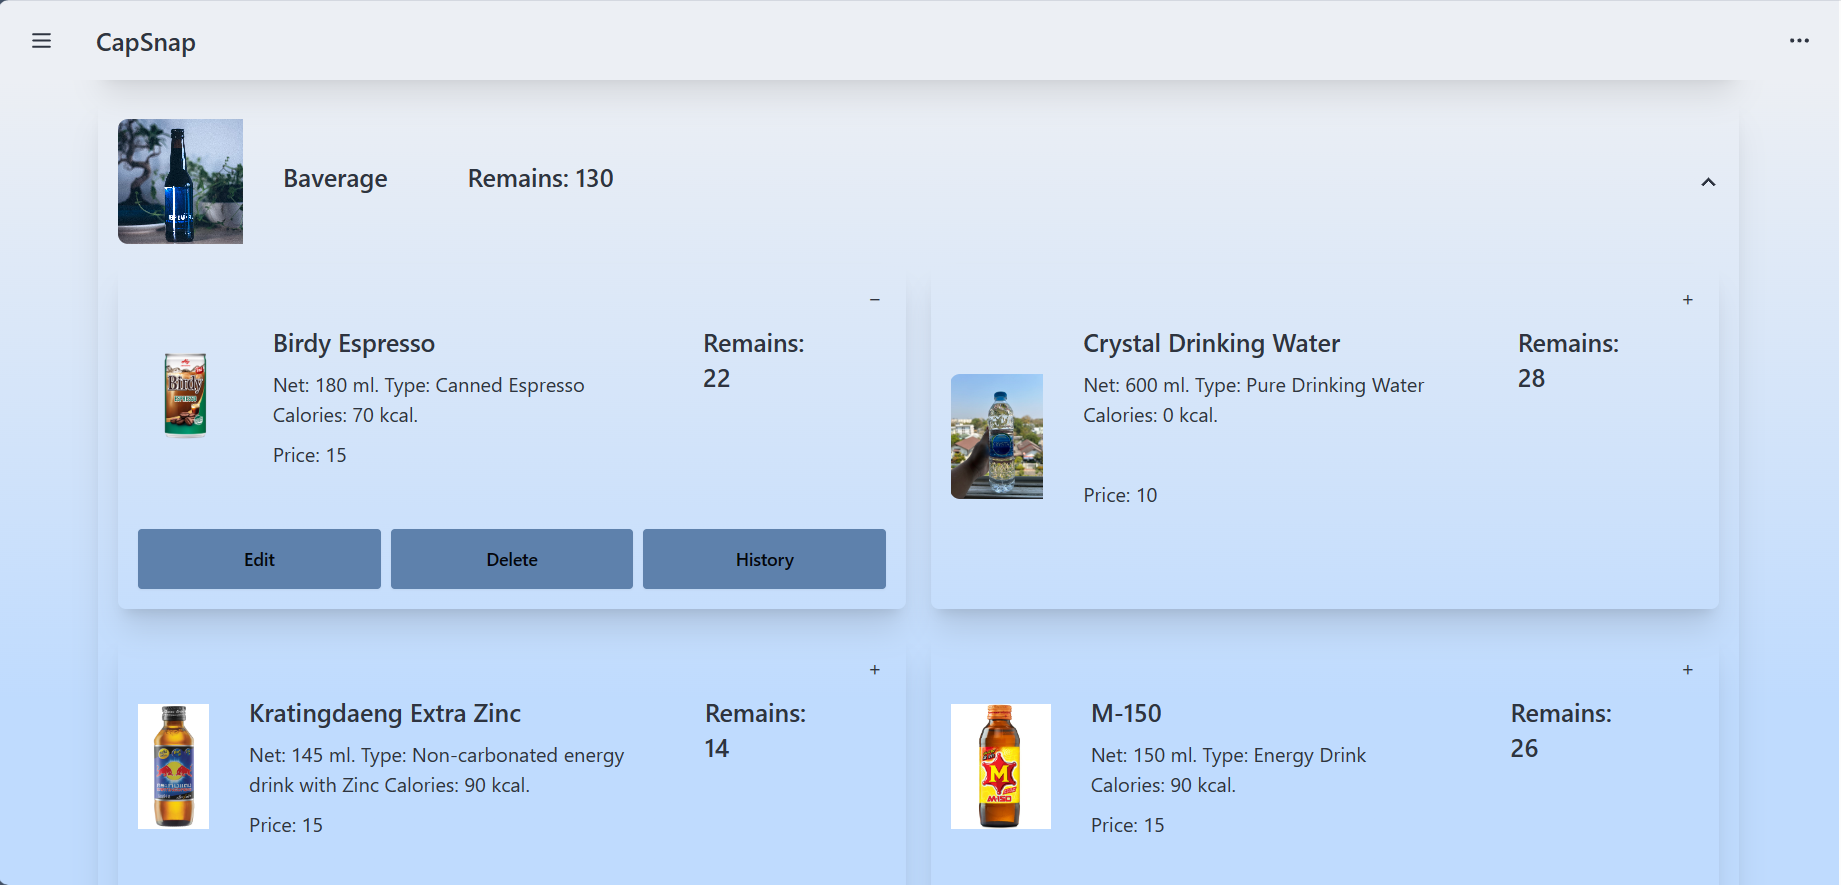
\includegraphics[scale=0.35]{pic/ui/w11.png}
}\\
{
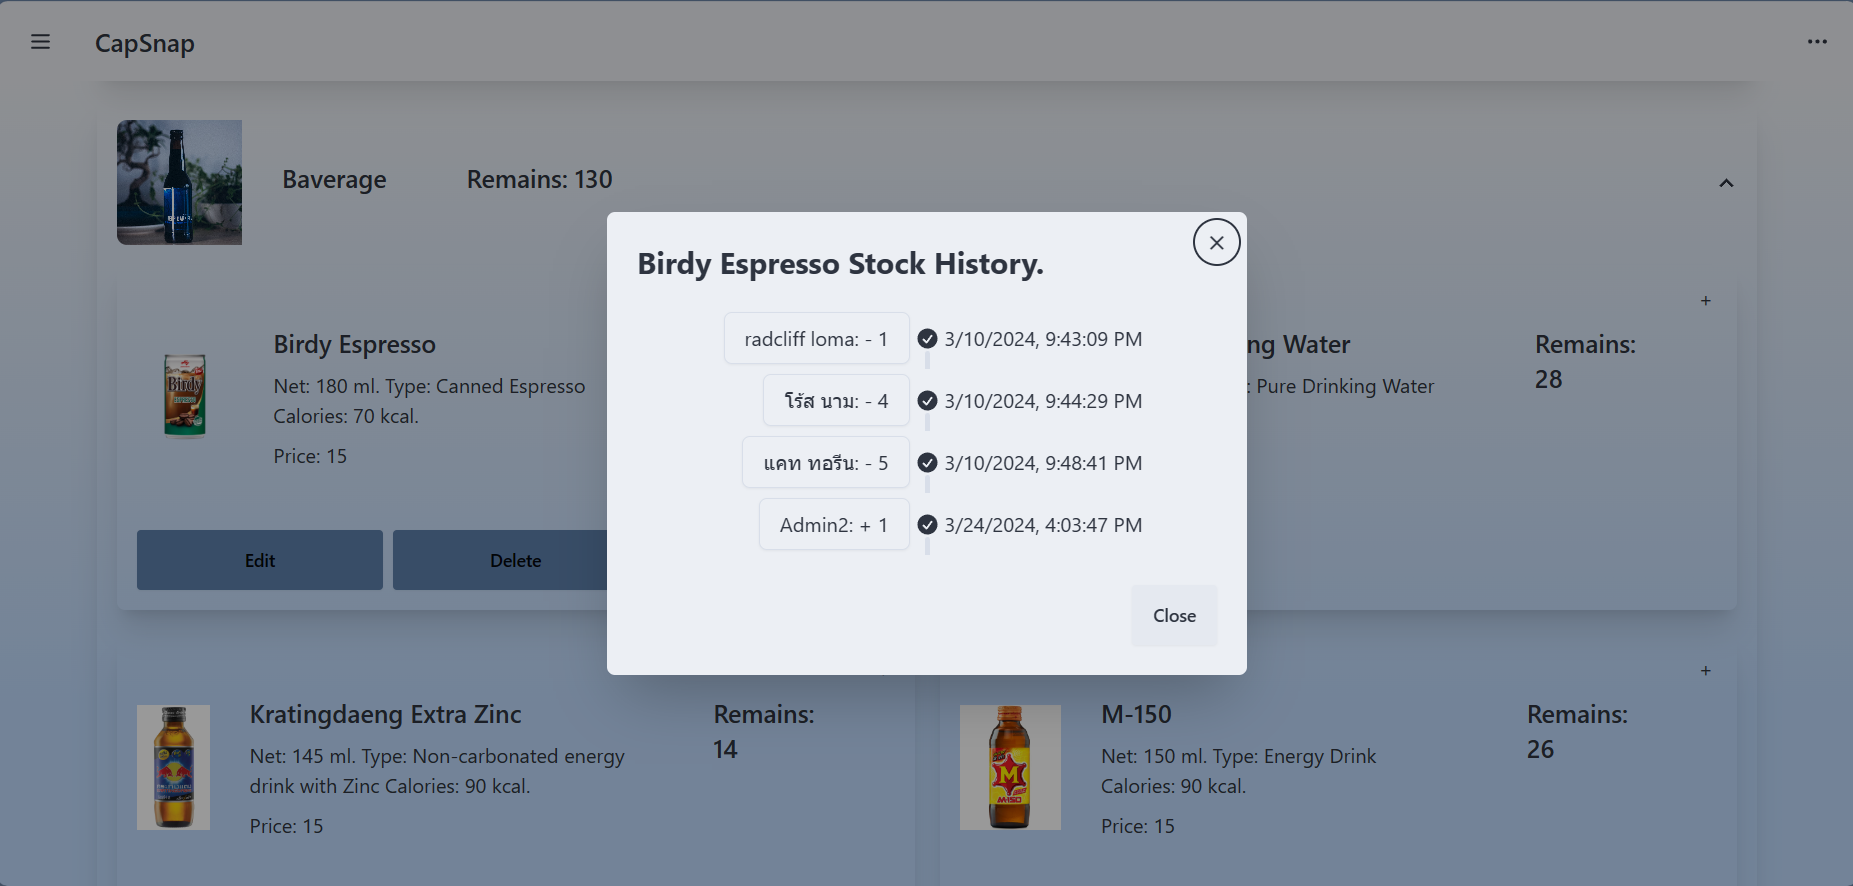
\includegraphics[scale=0.35]{pic/ui/w12.png}
}\\
{
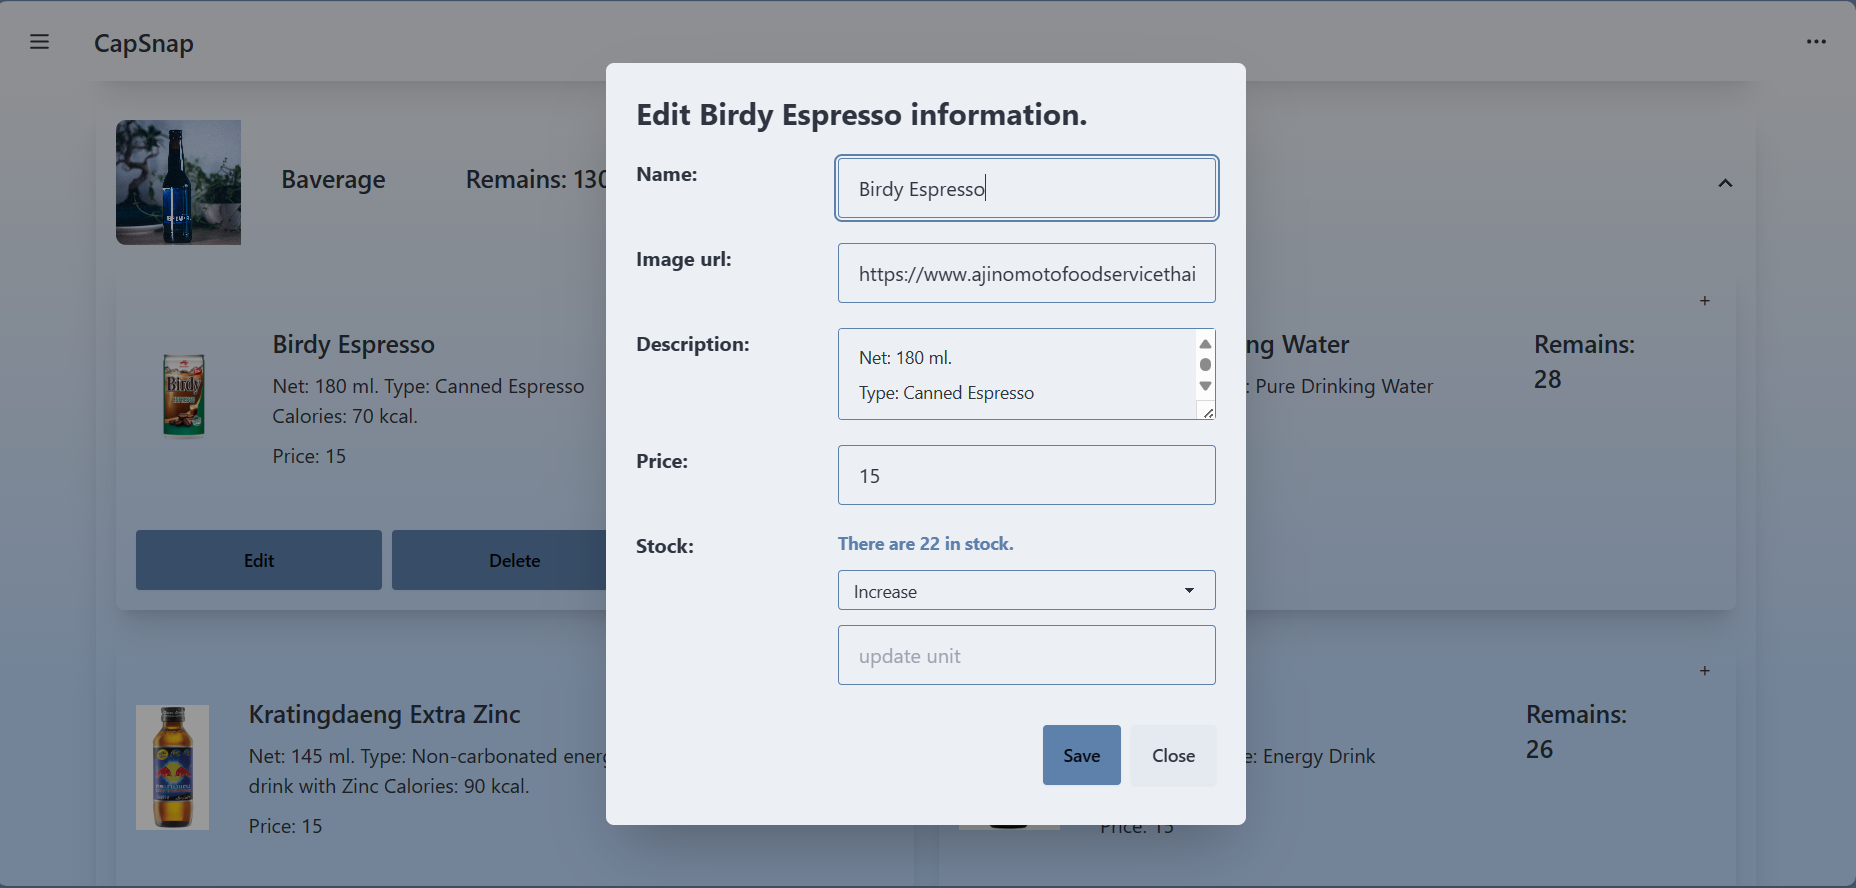
\includegraphics[scale=0.35]{pic/ui/w13.png}
}\\
{
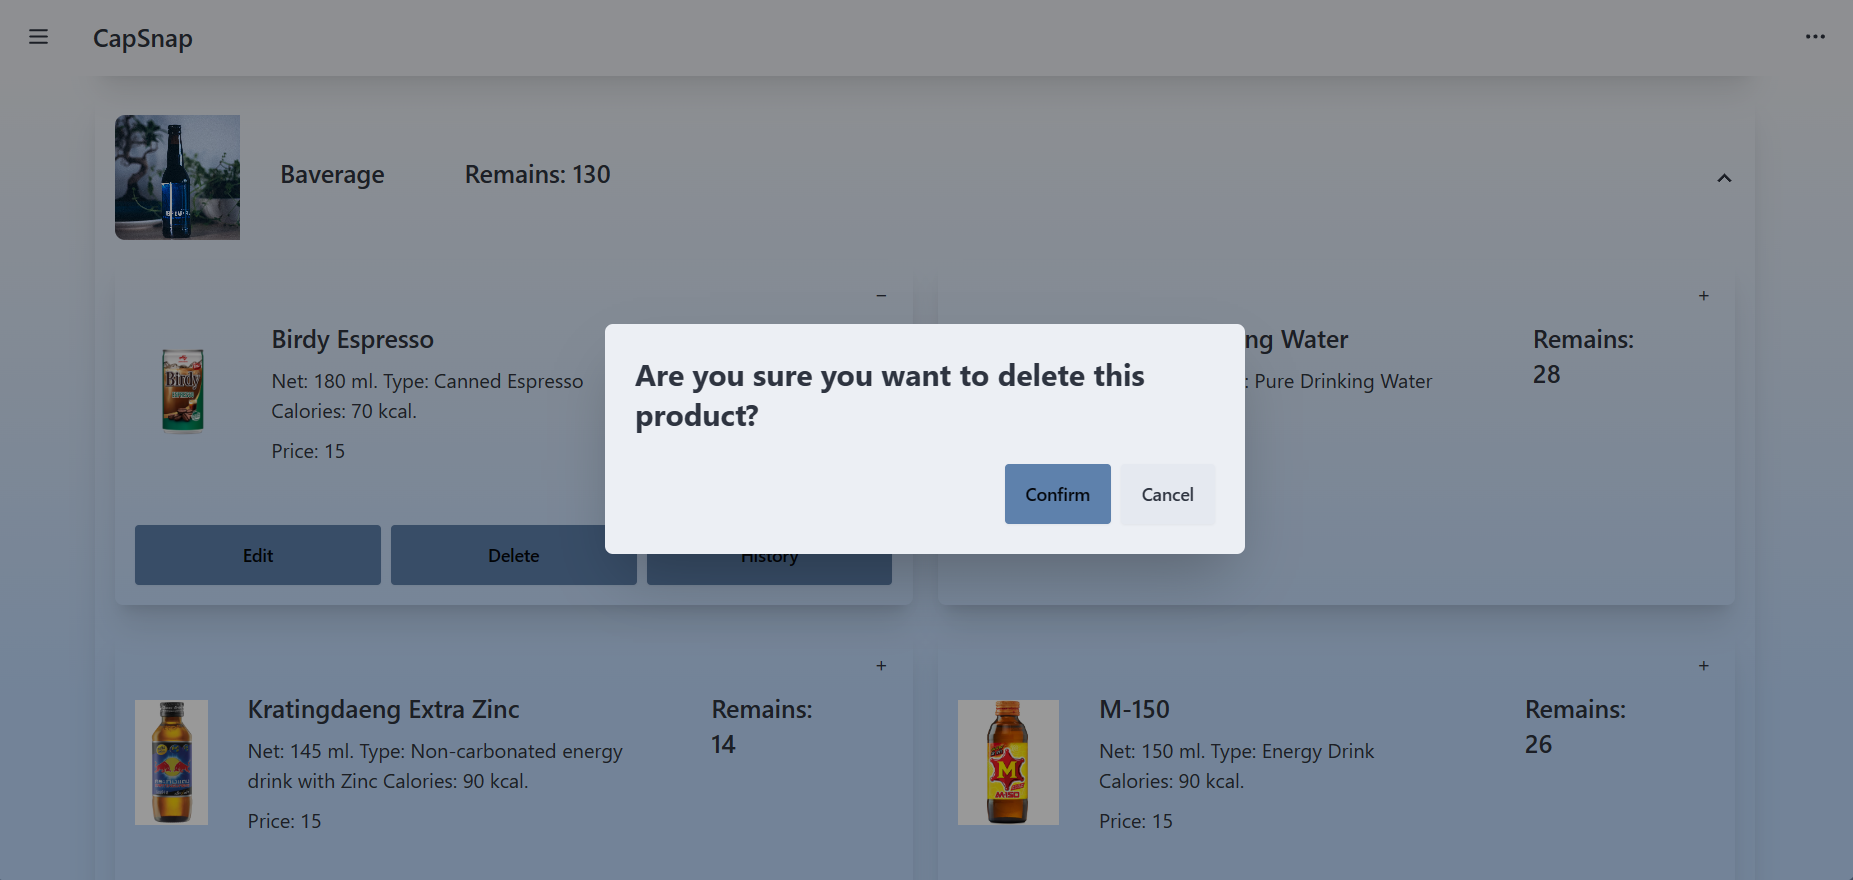
\includegraphics[scale=0.35]{pic/ui/w14.png}
}\\
\subsection{หน้าแสดงรายงานยอดขายสินค้า (Selling Report)}
เมื่อโหลดหน้าใหม่จะแสดงข้อมูลยอดขายของวันที่ปัจจุบันผ่านการ์ดข้อมูล แผนภูมิ และตาราง ในโหมดรายวัน ตามสินค้าทั้งหมด สามารถเลือกวันที่ที่ต้องการ และเปลี่ยนการแสดงผลตามรายวัน รายสัปดาห์ รายเดือน และรายปี ตามหมวดหมู่ของสินค้า หรือตามสินค้าทั้งหมดได้\\
{
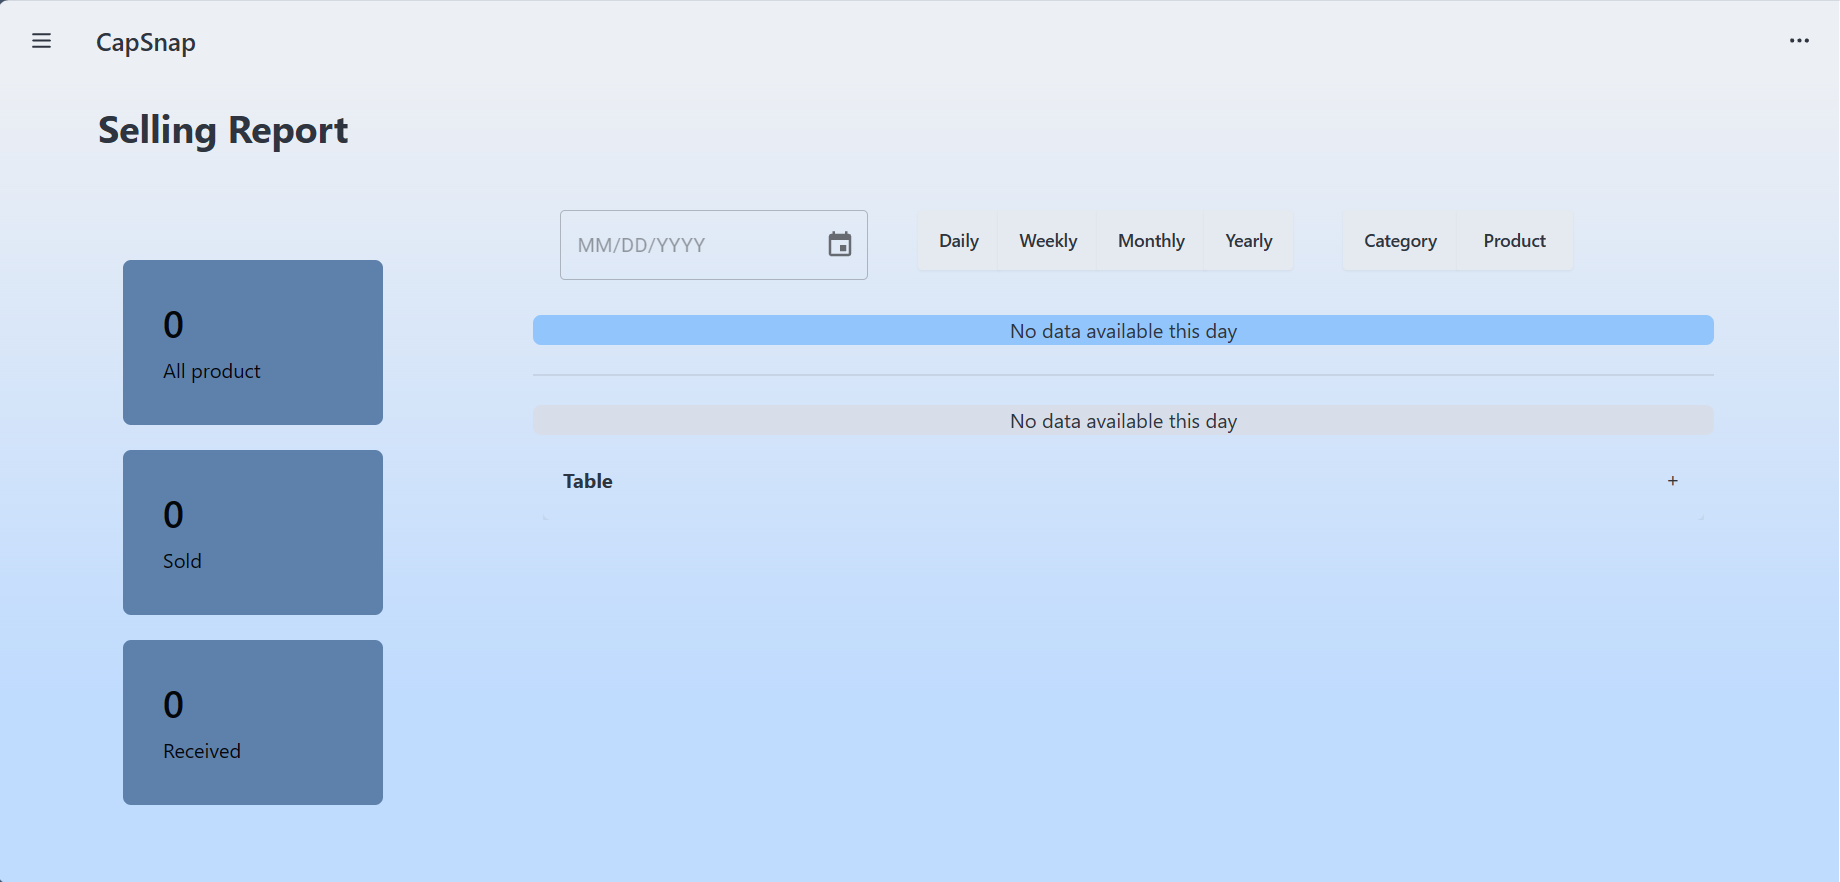
\includegraphics[scale=0.35]{pic/ui/w15.png}
}\\
{
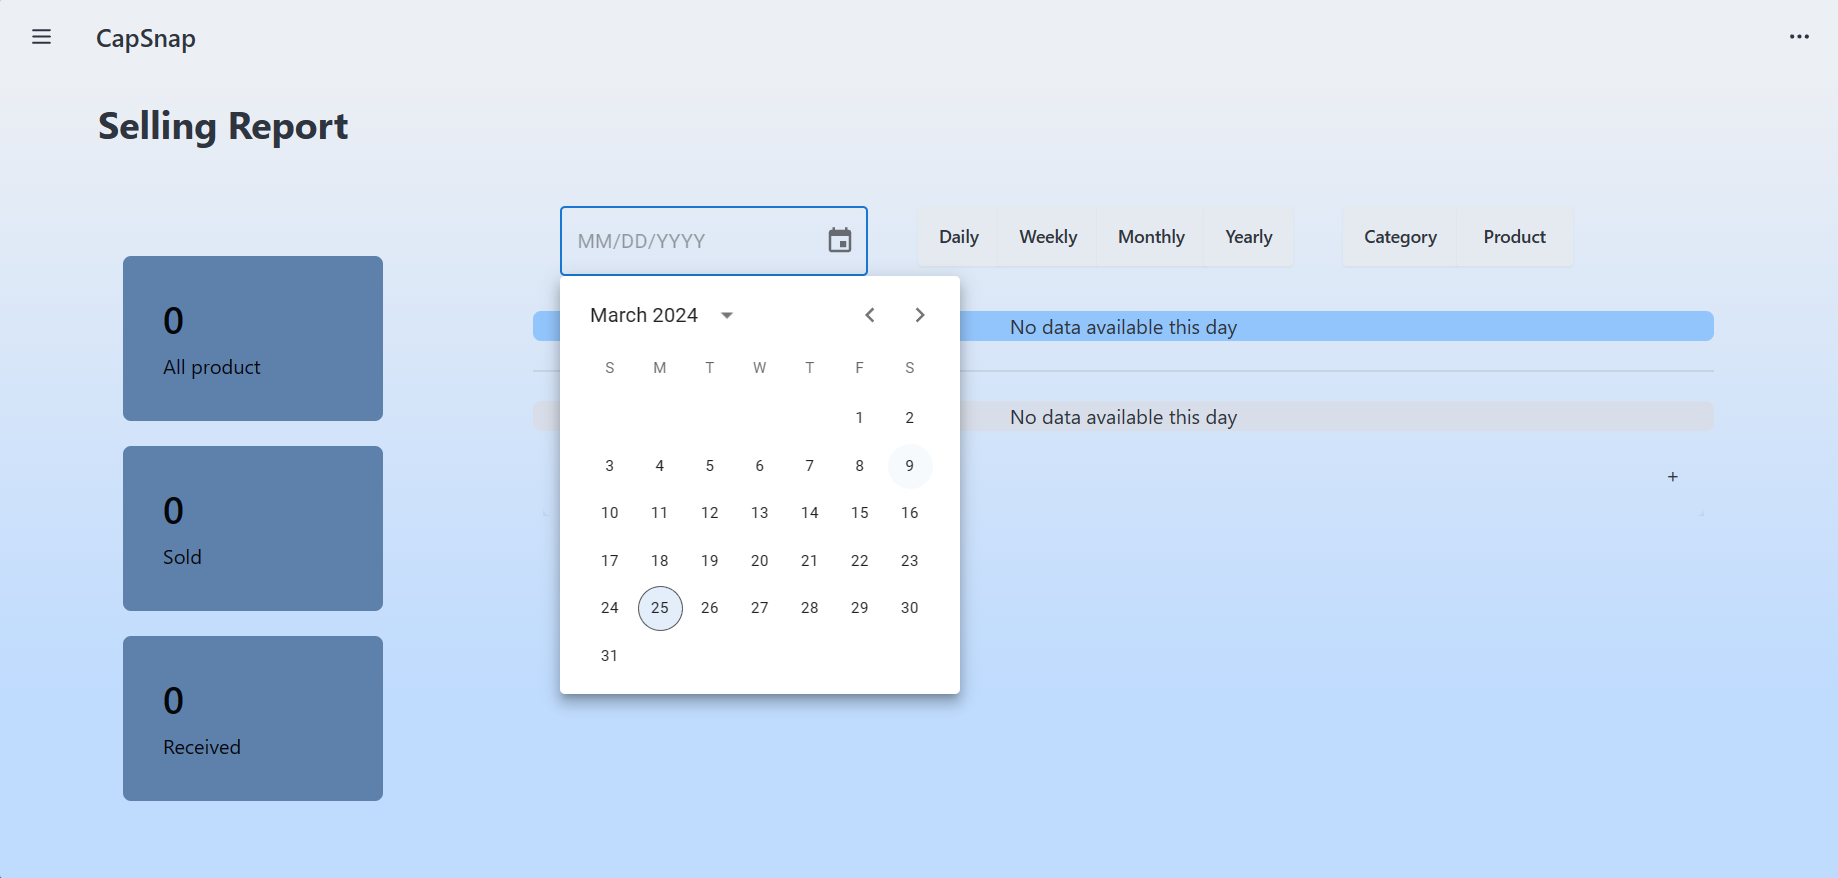
\includegraphics[scale=0.35]{pic/ui/w16.png}
}\\
{
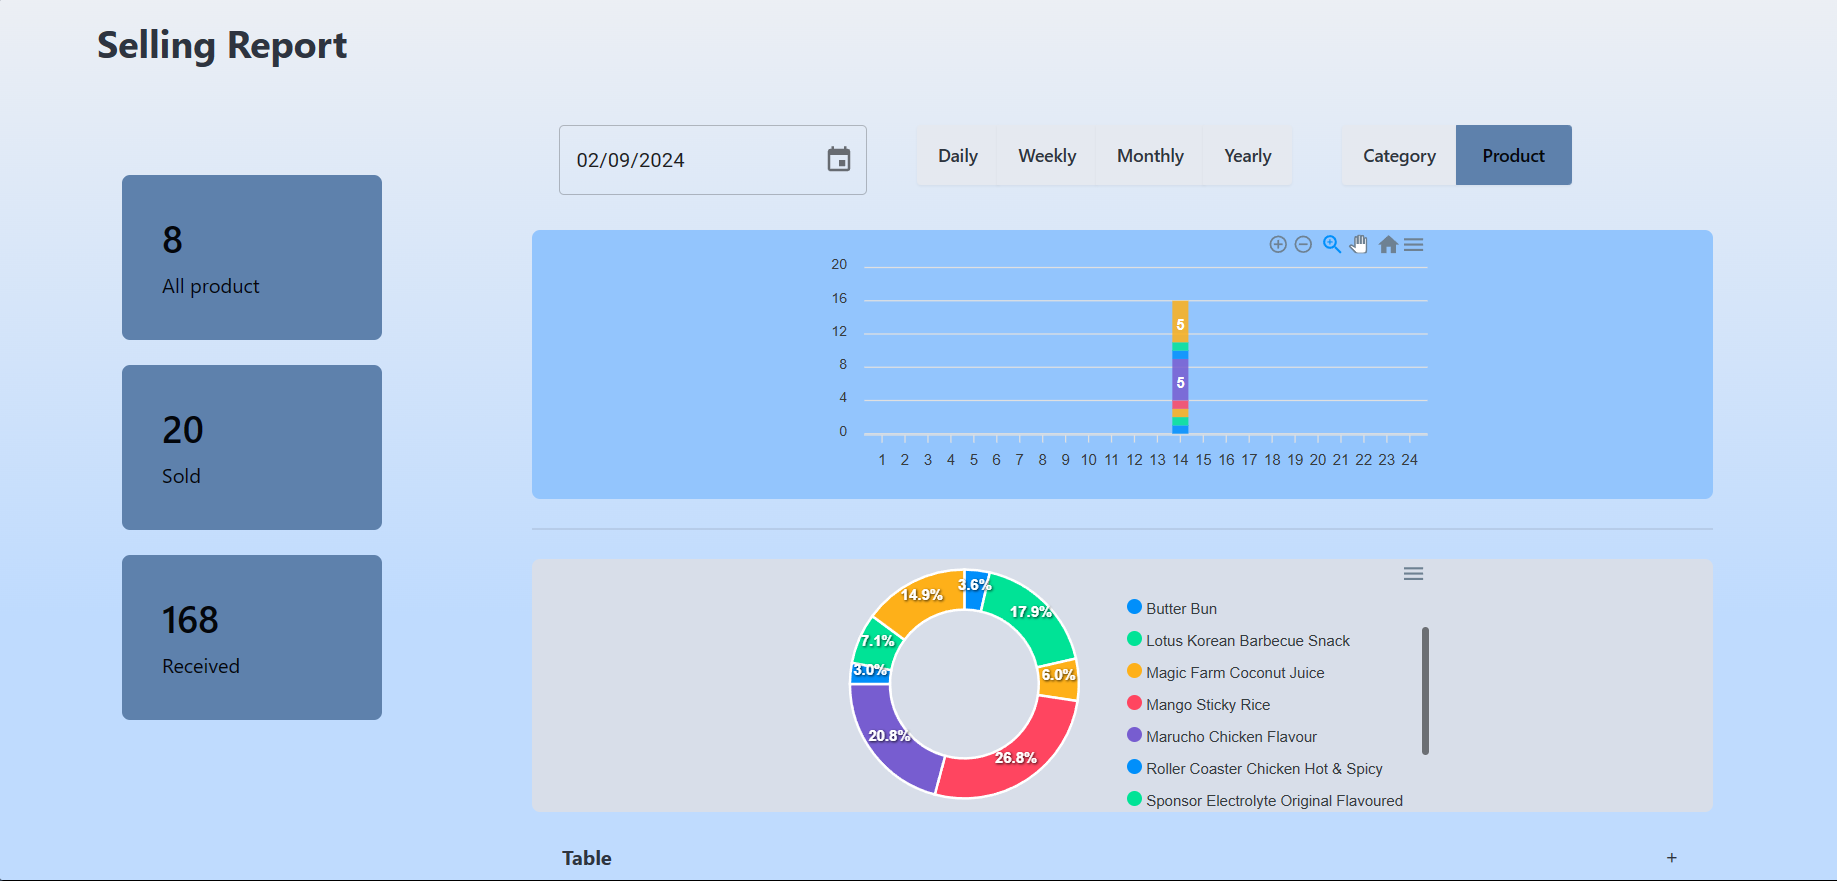
\includegraphics[scale=0.35]{pic/ui/w17.png}
}\\
{
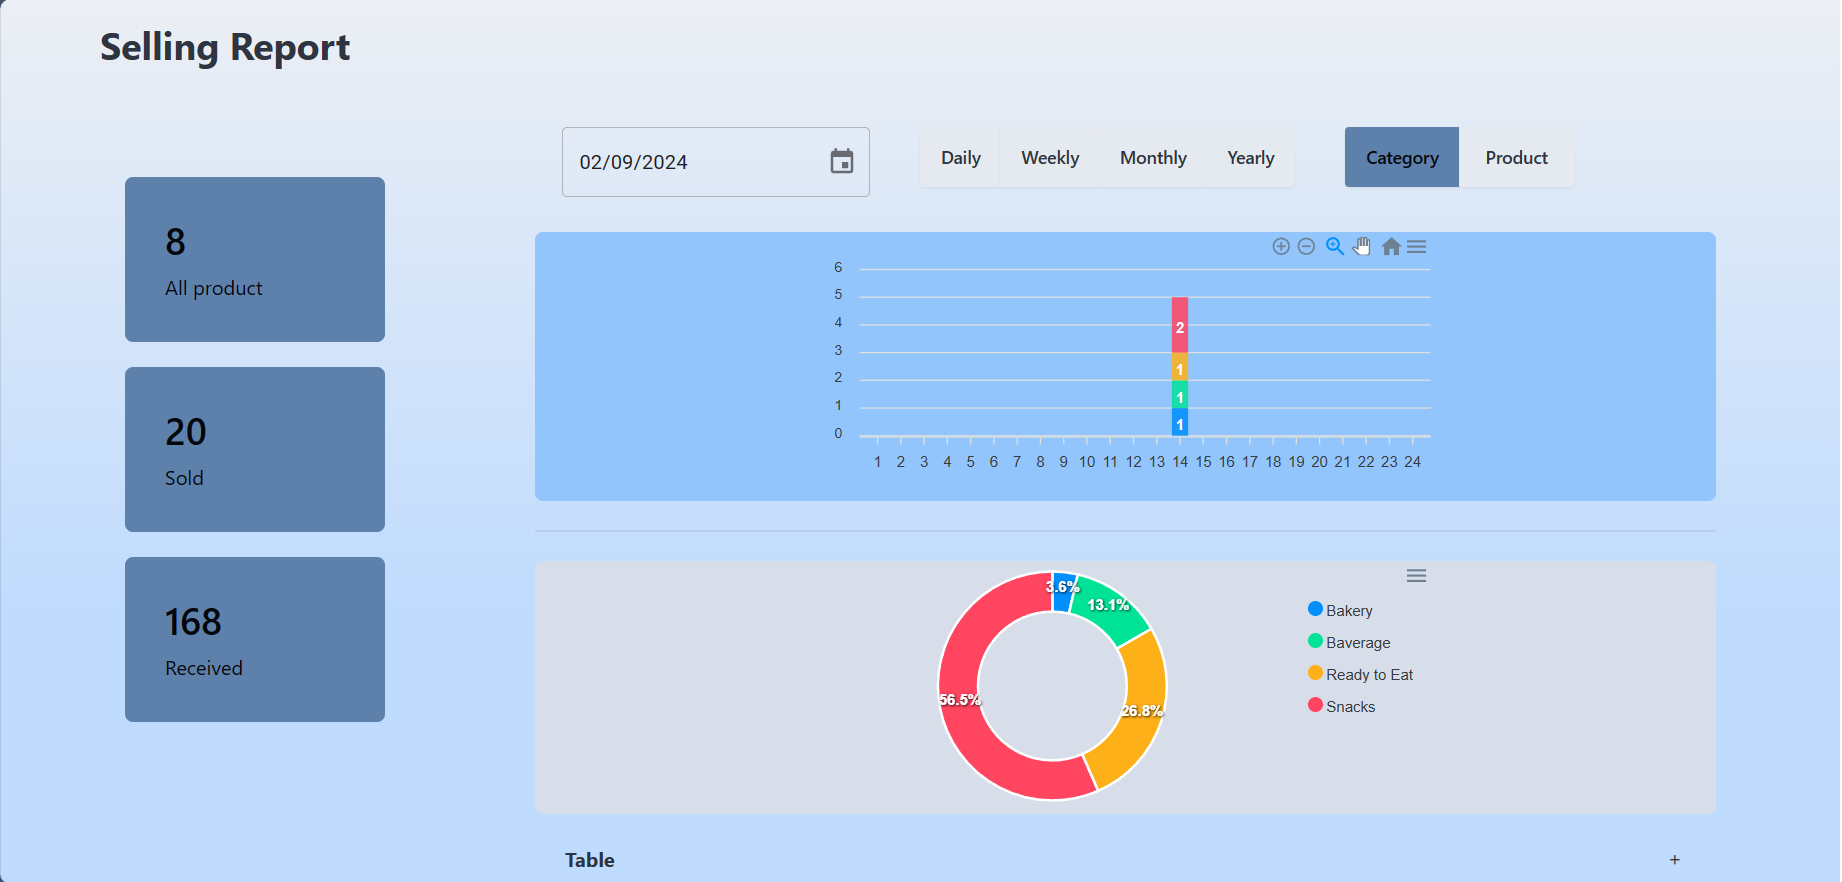
\includegraphics[scale=0.35]{pic/ui/w18.png}
}\\
{
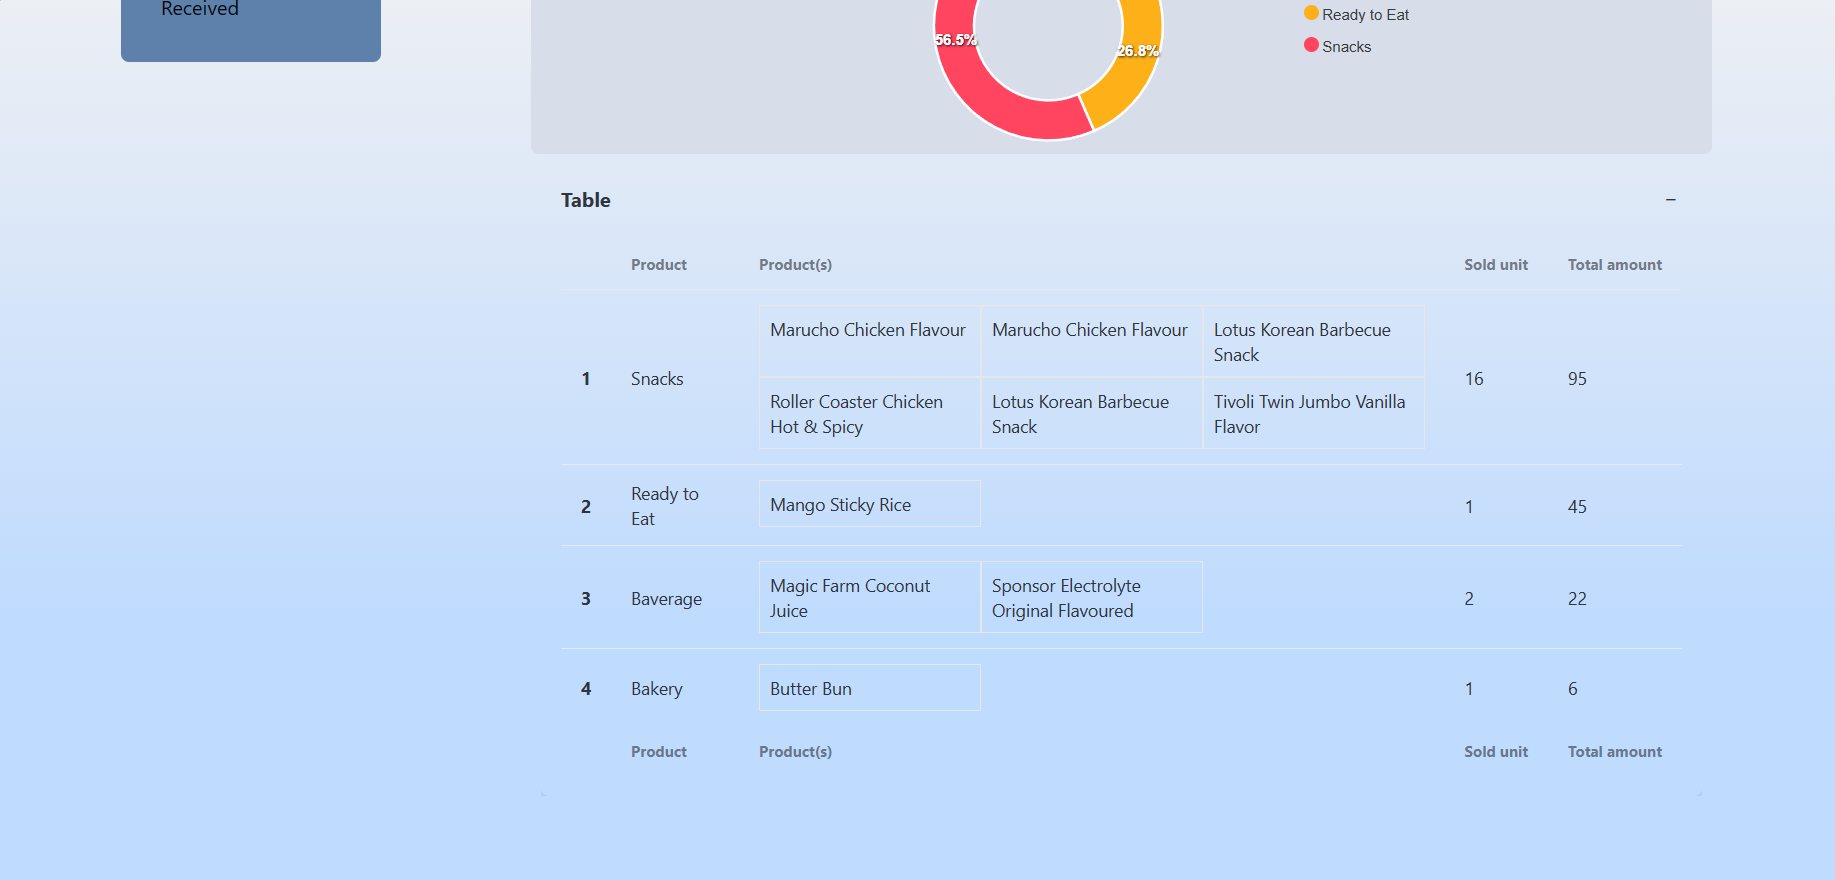
\includegraphics[scale=0.35]{pic/ui/w19.png}
}\\
{
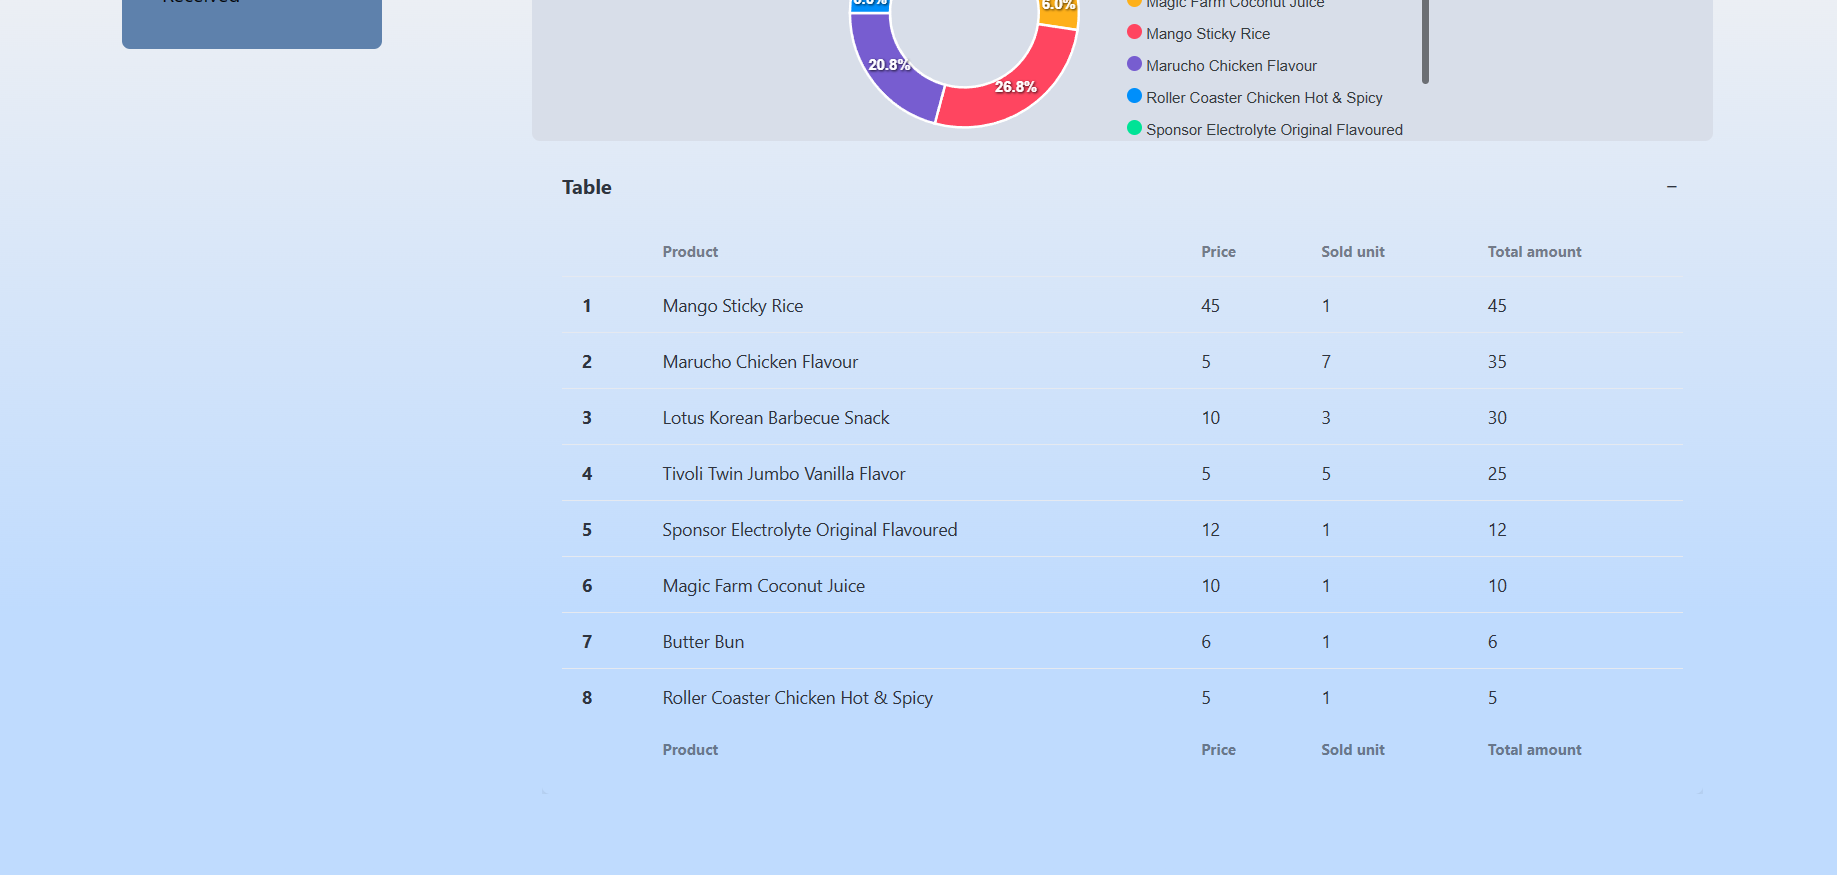
\includegraphics[scale=0.35]{pic/ui/w20.png}
}\\
{
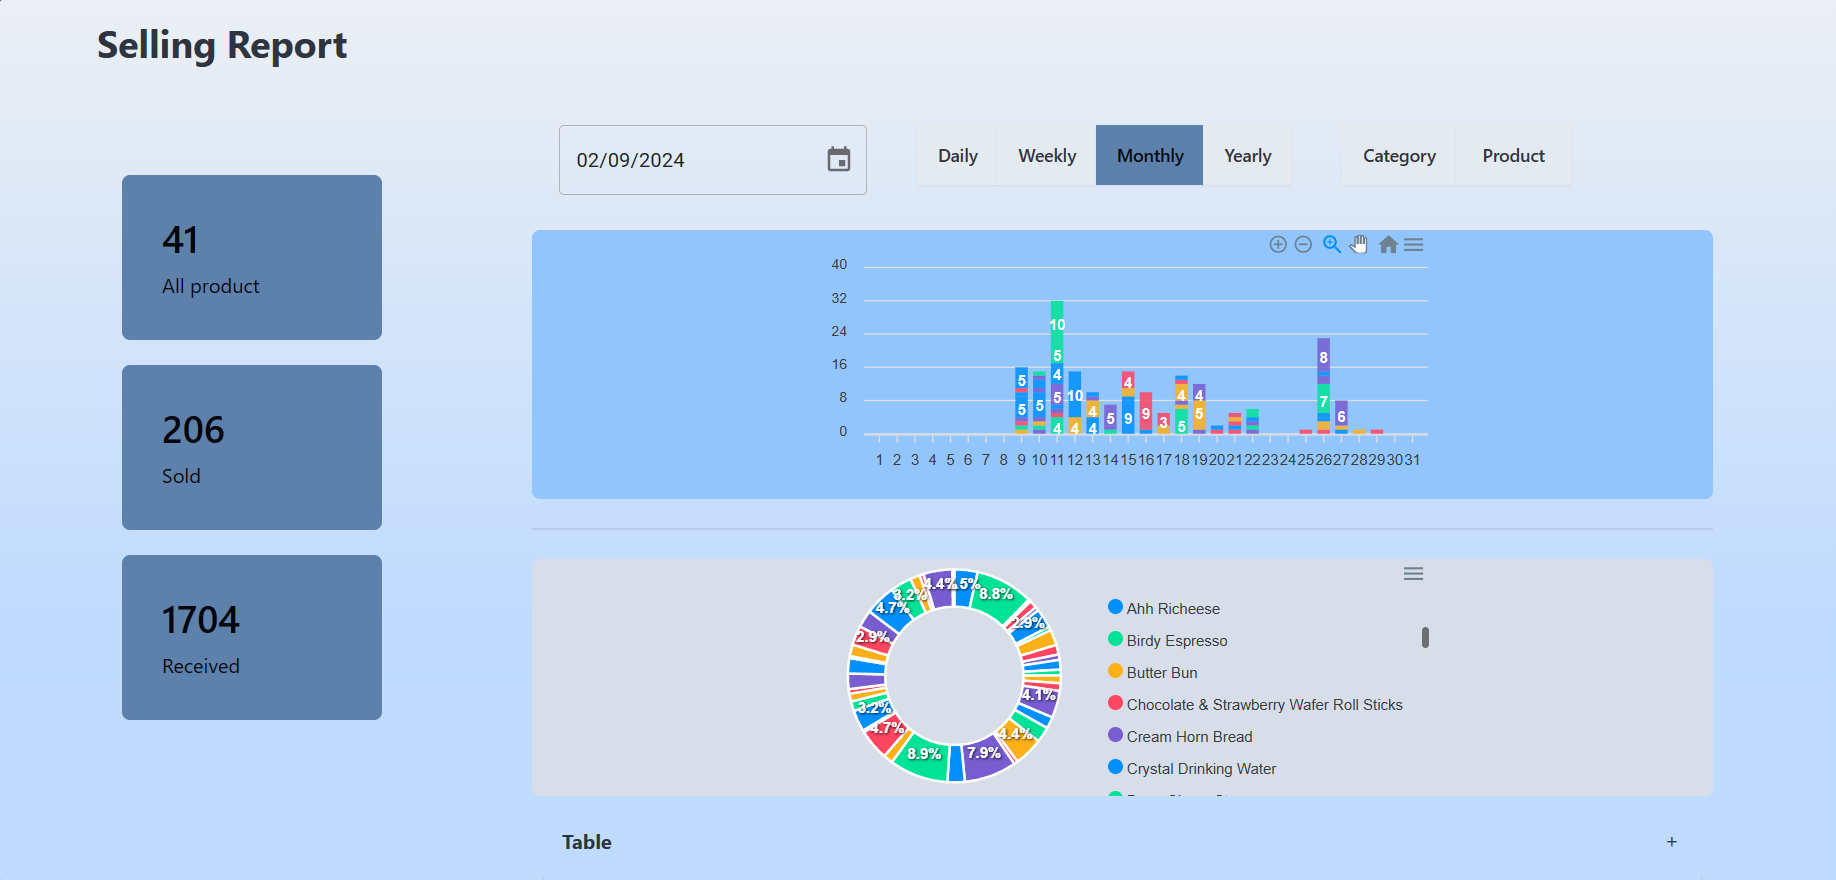
\includegraphics[scale=0.35]{pic/ui/w21.png}
}\\
{
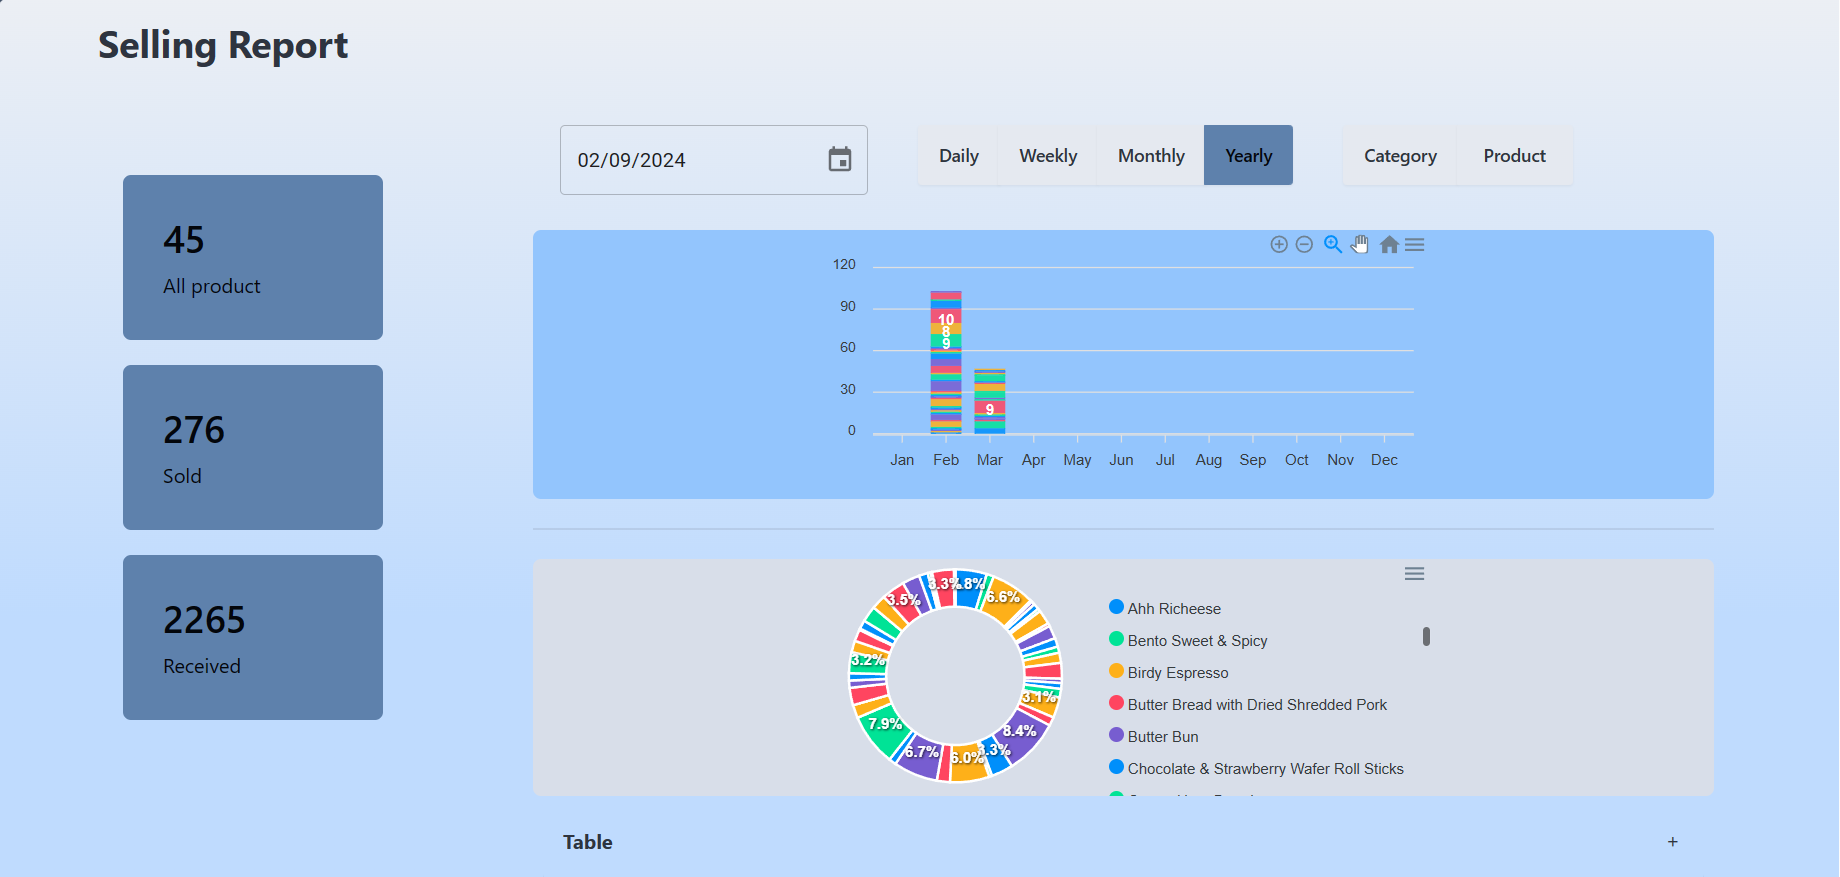
\includegraphics[scale=0.35]{pic/ui/w22.png}
}\\
\subsection{หน้าแสดงประวัติการซื้อสินค้าของลูกค้า (Purchase History)}
สำหรับหน้านี้จะแสดงรายการการซื้อของลูกค้าแต่ละครั้งในรูปแบบการ์ด ประกอบไปด้วยชื่อ วัน และเวลาที่ซื้อ และจำนวนเงินที่จ่าย เมื่อกดที่การ์ดจะแสดงรายการสินค้าที่ซื้อ จำนวนที่ซื้อ และราคาของสินค้าแต่ละชิ้น\\
{
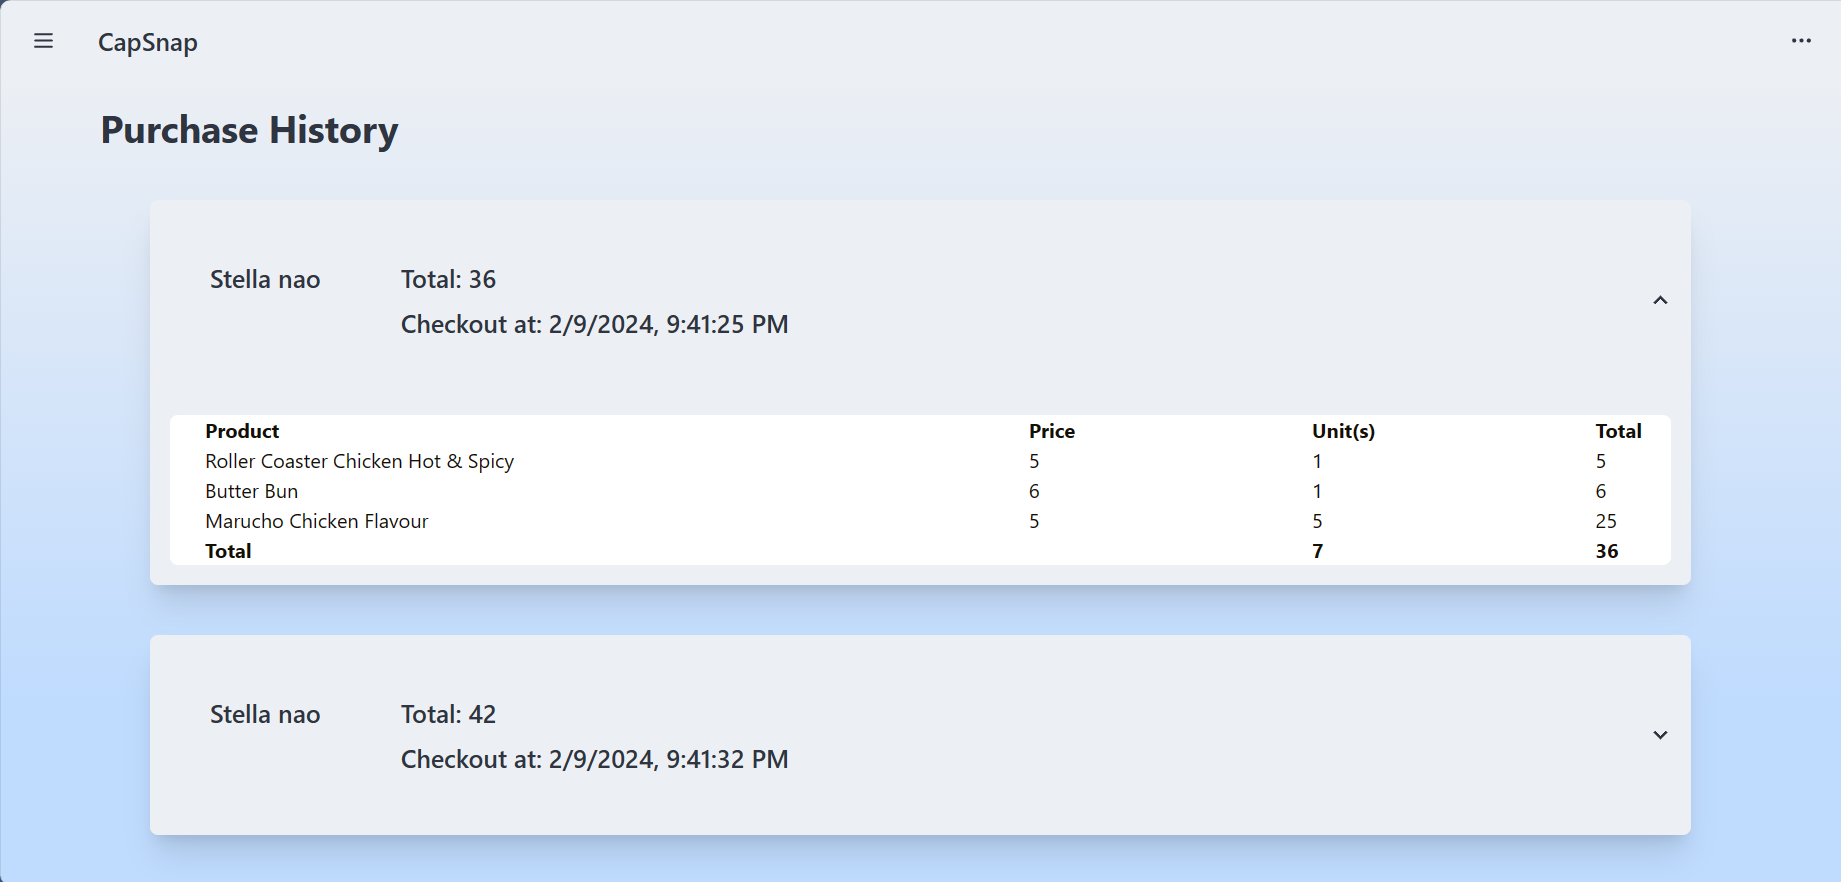
\includegraphics[scale=0.35]{pic/ui/w23.png}
}\\
\subsection{หน้าแสดงข้อมูลลูกค้า (Customers)}
สำหรับหน้านี้จะแสดงข้อมูลของลูกค้าแต่ละคนผ่านตาราง ได้แก่ ชื่อลูกค้า วันเกิด วันที่ลงทะเบียน และอีเมล์ และผ่านการ์ดข้อมูล ได้แก่จำนวนลูกค้าทั้งหมด จำนวนลูกค้าที่ลงทะเบียนใหม่ใน 7 วันที่ผ่านมา\\
{
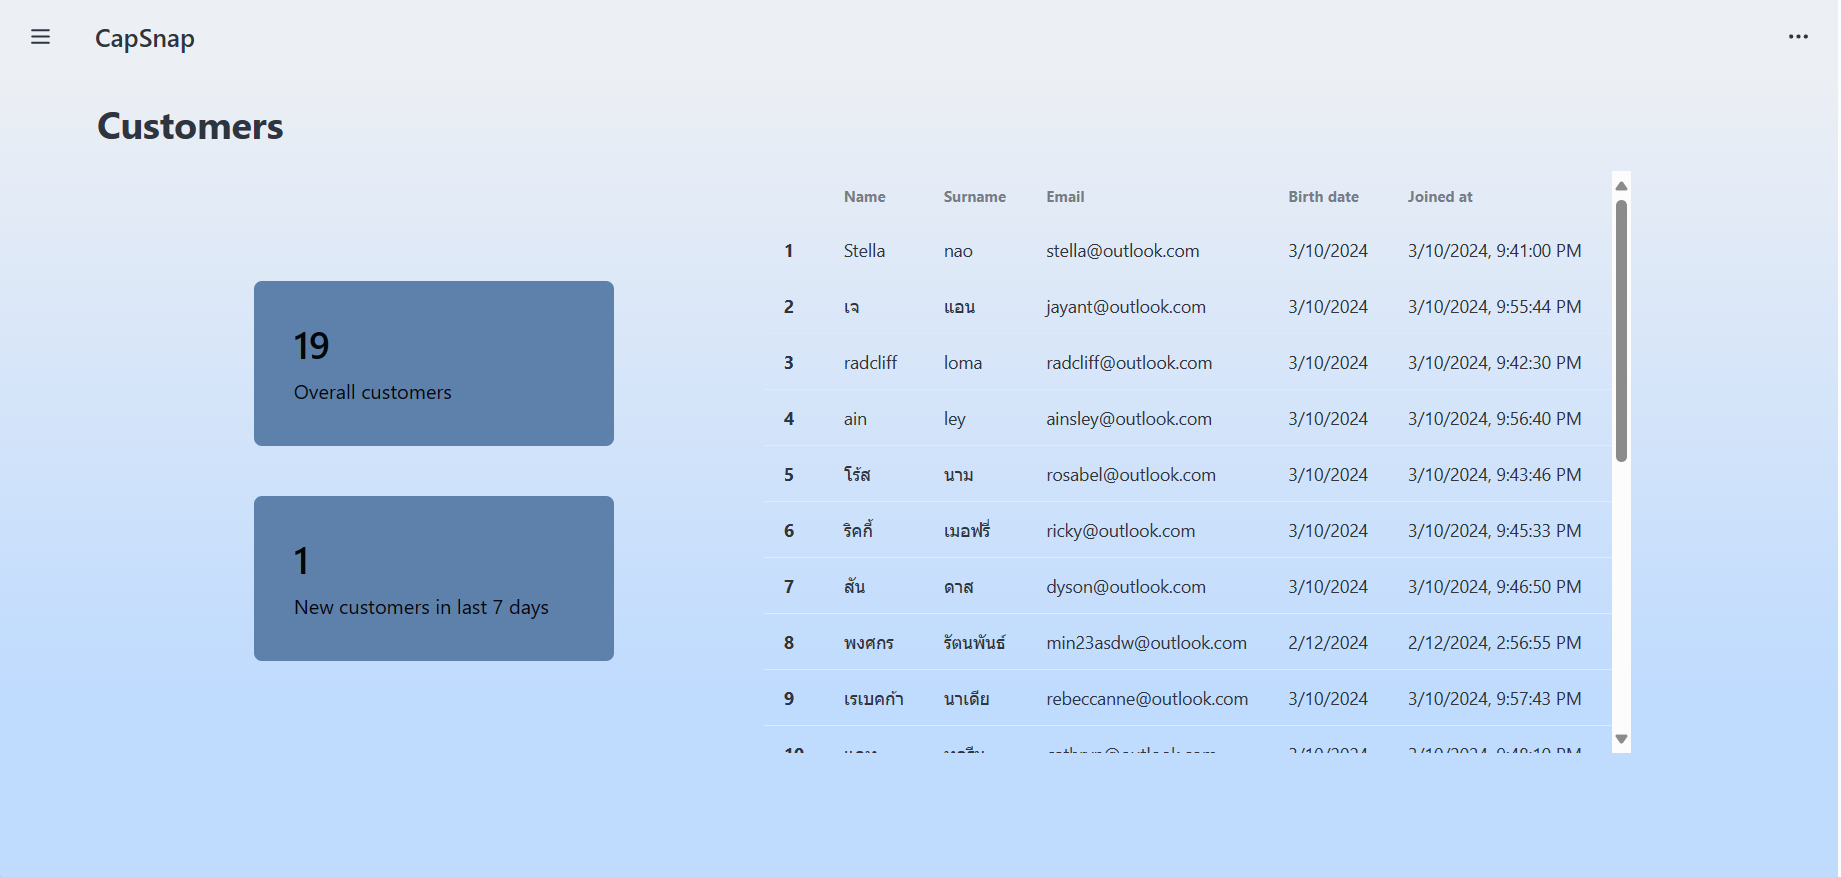
\includegraphics[scale=0.35]{pic/ui/w24.png}
}\\


% ในส่วนของการออกแบบส่วนสื่อประสานกับผู้ใช้ (GUI) ของ Website Dashboard นั้น ได้มีการพัฒนาตามที่ออกแบบไว้ แต่มีการปรับเปลี่ยนดีไซน์ และสีของหน้าเล็กน้อย แสดงผลลัพธ์การใช้งานได้ดังนี้
% \begin{enumerate}
%     \item Get started page: หน้าการเข้าสู่ระบบ หรือลงทะเบียนเข้าใช้งาน
%     \item Login page: หน้าการเข้าสู่ระบบ
%     \item Home page:  หน้าแสดงเมนูของฟังก์ชันต่าง ๆ
%     \item Menu bar:  แสดงเมนูของฟังก์ชันต่าง ๆ
%     \item Stock manager page: หน้าการจัดการคลังสินค้า
%     \item Stock manager page > Add new category: หน้าต่างการเพิ่มประเภทสินค้าใหม่
%     \item Stock manager page > Delete category: หน้าต่างการลบประเภทสินค้า
%     \item Stock manager page > Add new product: หน้าต่างการเพิ่มสินค้าใหม่
%     \item Stock manager page > Get product stock history: หน้าต่างการเพิ่มติดตามประวัติคลังสินค้า
%     \item Stock manager page > Delete product: หน้าต่างการลบสินค้า
%     \item Stock manager page > Edit product: หน้าต่างการแก้ไขสินค้า
%     \item Selling report page: หน้าการแสดงผลข้อมูลยอดขายตามรายวัน รายเดือน และรายปี โดยสามารถดูตามหมวดหมู่ของสินค้า หร���อแยกตามสินค้าหนึ่ง ๆได้
%     \item Selling report page > Date Time Picker: เลือกวันที่ต้องการติดตามรายงานยอดขาย
%     \item Selling report page > Graph: แสดงรายงานยอดขายผ่านแผนภาพ
%     \item Selling report page > Table: แสดงรายงานยอดขายผ่านตารางจากมากไปน้อย
%     \item Purchase History page: หน้าการติดตามประวัติการซื้อของลูกค้า
%     \item Customer page: หน้าแสดงข้อมูลของลูกค้าที่ลงทะเบียนผ่านโมบายแอปพลิเคชัน
% \end{enumerate}


% \end{center}

